\documentclass[letterpaper,12pt,oneside]{book}
\PassOptionsToPackage{hyphens}{url}

\usepackage{amsmath}
\usepackage{booktabs}
\usepackage[T1]{fontenc}
\usepackage[letterpaper]{geometry}
\usepackage[hidelinks]{hyperref}
\usepackage{listings}
\usepackage{mathptmx}
\usepackage{microtype}
\usepackage{multirow}
\usepackage[square,comma,numbers,sort&compress]{natbib}
\usepackage{setspace}
\usepackage{times}
\usepackage{tikz}
\usepackage{xspace}
\usepackage{amssymb}

\input{glyphtounicode}
\pdfgentounicode=1
\usetikzlibrary{arrows,arrows.meta, shapes.geometric,decorations.pathreplacing,calc,positioning}
\pagestyle{empty}
\doublespacing
\renewcommand{\ttdefault}{pxtt}
%\setcounter{secnumdepth}{-1}

\makeatletter
\renewcommand{\chapterautorefname}{\S\@gobble}
\makeatother

\newcommand{\sys}{\textsc{Ward}\xspace}
\newcommand{\contract}{\textsc{USC}\xspace}

\newcommand{\bench}{LEBench\xspace}

\newcommand*{\ditto}{---\textquotedbl---}
  
%% editing markup
\newcommand{\insertnote}[3]{\noindent\textcolor{#1}{\textbf{#2:} #3}}
\newcommand{\note}[1]{\insertnote{blue}{NOTE}{#1}}
\newcommand{\todo}[1]{\insertnote{red}{TODO}{#1}}
\newcommand{\jb}[1]{\insertnote{red}{JB}{#1}}
\newcommand{\ab}[1]{\insertnote{red}{AB}{#1}}
\newcommand{\fk}[1]{\insertnote{red}{FK}{#1}}
\newcommand{\nz}[1]{\insertnote{red}{NZ}{#1}}
\newcommand{\ac}[1]{\insertnote{red}{AC}{#1}}

\def\Snospace~{\S{}}
\def\sectionautorefname{\Snospace}
\def\subsectionautorefname{\Snospace}

\renewcommand{\topfraction}{0.9}
\renewcommand{\bottomfraction}{0.8}
\setcounter{topnumber}{2}
\setcounter{bottomnumber}{2}
\setcounter{totalnumber}{4}
\setcounter{dbltopnumber}{2}
\renewcommand{\dbltopfraction}{0.9}
\renewcommand{\textfraction}{0.07}
\renewcommand{\floatpagefraction}{0.7}
\renewcommand{\dblfloatpagefraction}{0.7}


\definecolor{codegreen}{rgb}{0,0.6,0}
\definecolor{codegray}{rgb}{0.5,0.5,0.5}
\definecolor{codepurple}{rgb}{0.58,0,0.82}
\definecolor{backcolour}{rgb}{0.95,0.95,0.92}
\lstdefinestyle{codeStyle}{
    backgroundcolor=\color{backcolour},   
    commentstyle=\color{codegreen},
    keywordstyle=\color{magenta},
    numberstyle=\tiny\color{codegray},
    stringstyle=\color{codepurple},
    basicstyle=\ttfamily\footnotesize,
    breakatwhitespace=false,         
    breaklines=true,                 
    captionpos=b,                    
    keepspaces=true,                 
    numbers=left,                    
    numbersep=5pt,                  
    showspaces=false,                
    showstringspaces=false,
    showtabs=false,                  
    tabsize=2,
    language=C++
}
\lstset{style=codeStyle}

\begin{document}

\begin{titlepage}
\newgeometry{top=1.5in,bottom=1in,right=1.25in,left=1.25in}

    \centering
    \onehalfspacing
    {\large \bf Understanding and Improving the Performance of Mitigating Transient Execution Attacks} \\[1\baselineskip]
    by \\[0.25\baselineskip]
    {\large Jonathan Behrens} \\[1\baselineskip]

    B.S., Cornell University (2016) \\
    S.M., Massachusetts Institute of Technology (2018) \\[1\baselineskip]

    Submitted to the Department of Electrical Engineering and Computer Science \\
    In Partial Fulfillment of the Requirements for the Degree of\\[0.5\baselineskip]

    Doctor of Philosophy

    at the 

    MASSACHUSETTS INSTITUTE OF TECHNOLOGY

    February 2022 \\[0.5\baselineskip]

    \copyright 2022 Massachusetts Institute of Technology. All rights reserved \\[0.25in]

    \singlespacing
    \raggedleft
    \small

    Signature of Author................................................................................................................................ \\
    Department of Electrical Engineering and Computer Science \\
    January 26, 2022 \\[1\baselineskip]

    Certified by ............................................................................................................................................. \\
    M. Frans Kaashoek \\
    Charles Piper Professor of Electrical Engineering and Computer Science \\
    Thesis Supervisor \\[1\baselineskip]

    Co-Certified by ...................................................................................................................................... \\
    Adam Belay \\
    Assistant Professor of Electrical Engineering and Computer Science \\
    Thesis Co-Supervisor \\[1\baselineskip]

    Accepted by ............................................................................................................................................ \\
    Leslie A. Kolodziejski \\
    Professor of Electrical Engineering and Computer Science \\
    Chair,  Department  Committee  on  Graduate  Students

\restoregeometry
\end{titlepage}
\setcounter{page}{2}
~\newpage


\singlespace
\begin{center}

{\large \bf Understanding and Improving the Performance of Mitigating Transient Execution Attacks} \\[.5\baselineskip]
by \\
Jonathan Behrens \\[.5\baselineskip]
\end{center}

Submitted to the Department of Electrical Engineering and Computer Science on January 26, 2022 in Partial Fullfillment of the Requirements for the Degree of Doctor of Philosophy in Electrical Engineering and Computer Science.\\[.5\baselineskip]

\noindent
ABSTRACT \\

This these makes two contributions:
(1) it measures the performance evolution of mitigations against transient execution side channel attacks over several generations of processors, and (2) introduces the \sys kernel design, which eliminates as much as half the overhead on older processors.

The measurement study maps end-to-end overheads to the specific mitigations that cause them.
It reveals that hardware fixes for several transient execution attacks have reduced overheads on OS heavy workloads by a factor of ten.
However, overheads for JavaScript applications have remained roughly flat because they are caused by mitigations for attacks that even the most recent processors are still vulnerable to.
Finally, the study shows that a few mitigations account for most performance costs.

% On workloads that stress the Linux kernel interface (which have received the most attention) there have been substantial improvements with slowdowns on the LEBench benchmark suite going from over 30\% to less than 3\%.
% By contrast, the overhead for JavaScript applications running inside Firefox are impacted by an almost entirely different set of mitigations which haven't gotten better with newer processors.

\sys is a novel operating system architecture that is resilient to transient execution attacks, yet avoids many of the expensive software mitigations that existing operating systems employ when running on pre-2018 processors.
It leverages a new hardware/software contract termed the Unmapped Speculation Contract, which describes baseline limits on the speculative behavior of processors.

~\\[\baselineskip]

\noindent
Thesis  Supervisor:  M.  Frans  Kaashoek \\
Title:  Charles  Piper  Professor  of Electrical  Engineering  and  Computer  Science \\[.5\baselineskip]
\noindent
Thesis  Supervisor:  Adam Belay \\
Title:  Assistant Professor  of Electrical  Engineering  and  Computer  Science \\

\doublespace
~\newpage


{\noindent \huge \bf Acknowledgments\\}

I want to extend my thanks to my advisors Frans Kaashoek and Adam Belay
for their guidance and mentorship, to my other committee members Nickolai Zeldovich and Mengjia Yan for their valuable feedback, and to all the past and present members of PDOS who I have learned so much from over these years.
Thank you.

I would also like to specifically thank all of my collaborators including Jack Cook, Jules Drean, Anton Cao, Cel Skeggs, Amy Ousterhout, Joshua Fried, Hari Balakrishnan, Jon Gjengset, Malte Schwarzkopf, Lara Timbó Araújo, Martin Ek, Eddie Kohler, Sagar Jha, Ken Birman, and Edward Tremel. Your insights and support have meant a ton.

I am extraordinarily thankful to my friends and family have supported me every step of this journey.
You have shaped my experiences, given me meaning and purpose, and helped me drive positive change.
I would not be where I am today without you.

\begin{center}
    ~\\[\baselineskip]
    $\star~\star~\star$
    ~\\[\baselineskip]
\end{center}


\noindent
This dissertation extends work from the following papers:
\begin{itemize}
\item Efficiently mitigating transient execution attacks using the unmapped speculation contract. \textit{OSDI 2020}.
\item Performance Evolution of Mitigating Transient Execution Attacks. To appear. \textit{\mbox{EuroSys} 2022}.
\end{itemize}

~\newpage

\pagestyle{plain}
\tableofcontents

\chapter{Introduction}
\noindent
Side channel attacks leak information between isolation domains outside of the normal information flow of a system.
Several years ago a new class of side channel attacks was discovered impacting CPUs from all major vendors~\cite{lipp:meltdown, kocher:spectre}.
These attacks -- termed transient execution attacks -- exploit details of how modern processors use speculative execution to run more quickly. 

Transient execution attacks represent a concern for operating system developers because a key security responsibility for operating systems is to maintain isolation.
In particular, multiple processes running on the same machine must not inadvertently leak information between one another.
Production operating systems and other software vendors have deployed a range of software techniques devised to mitigate the impact of these attacks, but unfortunately they introduce significant performance trade offs.

The overhead caused by these mitigations is present on the many hundreds of millions vulnerable processors dating from before the discovery of the attacks, and also at least to some degree on all major commercial CPUs released after their discovery.
This thesis both attempts to quantify how this overhead has evolved over subsequent generations of processors and presents an operating system design to reduce OS level overheads on the CPUs where they are most severe.  

% Many hundreds of millions of vulnerable computer processors are currently in use, so simply replacing them all isn’t by itself a viable solution.
% Worse still, computer architectural approaches to solve transient execution attacks remains an open area of research, except on the simplest of processors.

% Nonetheless, generations of processors designed after the discovery of transient execution attacks have improvements that make them inherently less susceptible to attack.
% It is desirable to understand how this was achieved yet little has been published on exactly what changes were made.
% The focus of this thesis is on understanding and reducing the impact of mitigations on performance.

\section{Transient Execution Attacks}
\subsection{Speculative Execution}
Speculative execution is an optimization used in the design of modern processors to drastically improve their performance, by enabling them to do useful work during times when they would otherwise be stalled waiting to load information from RAM.
When the CPU reaches a conditional branch instruction that it doesn't yet know whether will be taken or not, it predicts the outcome and then starts executing instructions that would follow.
The prediction is based on prior executions of that same instructions and any other heuristics the processor may have.

Usually the branch prediction is correct and the speculatively executed instructions can be committed.
However, when the prediction is incorrect, the CPU rolls back the architecturally visible results of the instructions executed after the branch.
In general when reverting transiently executed instructions, their microarchitural effects -- like inserting or evicting lines from the cache -- are not undone.
Observing the  microarchitural effects of speculatively executed instructions is the core of transient execution attacks.

\subsection{Example Attack}
\begin{figure}[h]
\begin{lstlisting}[language=C, style=codeStyle]
if (index < array_size) {
    int v = array2[array1[index] * 256];
    ...
}
\end{lstlisting}
\caption{Example code for a Spectre V1 attack}
\label{fig:spectre-code}
\end{figure}
Spectre V1 was one of the earliest attacks discovered and leaks information between different processes, between a process and the operating system kernel, or between a sandbox and the code running within.
The attack relies on a specific sequence of instructions (a ``gadget'') to be located in the victim's code region.
The gadget consists of a bounds check followed by two array accesses as shown in Figure~\ref{fig:spectre-code}, for which the index value can be controlled by the adversary.

To trigger the attack, the adversary will repeatedly call the gadget with in bounds indexes.
This will train the CPU branch predictor that the branch is usually taken.
Then, the attackers forces the array size to be evicted from the CPU cache and calls the gadget with an out of bounds index.

When execution reaches the bounds check, the processor will initiate a load to read the array size.
However before that load completes, the CPU will speculatively start executing the body of the if statement because the branch predictor has previously learned that the index is usually in bounds.
The first array access will read past the end of the array into arbitrary memory and pull that value into a CPU register.
The second array access then loads a specific cache line whose index will depend on the first read.

Eventually the branch misprediction will be discovered and rolled back, but the cache contents will not be.
This enables the attacker to later time how long it takes to access each cache entry and infer which value must have been pulled in by the victim application.

\subsection{Other Attacks}
There are a whole range of other transient execution attacks which can be divided into three categories~\cite{hill:survey}.
Spectre type attacks like the one described above rely on processor misprediction to incompletely roll back executed instructions.
Meanwhile Meltdown type attacks achieve the same effect using a trapping operation to trigger the roll back.
Finally, Microarchitural Data Sampling exploits the processor's forwarding logic to cause the processor to erroneously run instructions with data fed from a sibling hyperthead or previously running task, rather than the correct values.

\section{Mitigation Approaches}
\subsection{Software}
As the embargo period wound down on the original Meltdown and Spectre attacks, operating system vendors and processor makers hurriedly rolled out patches to mitigate these vulnerabilities.
The patches came at a significant performance cost. 

These fixes took two forms.
Hardware vendors released microcode patches for existing processors which modified behavior and added some new functionality to control speculative execution~\cite{intel:l1tf}.
Meanwhile, operating system makers and other software vendors deployed new versions which blocked the attacks via a combination of software only techniques~\cite{intel:retpoline, linux:kpti} and leveraging the functionality added by microcode~\cite{intel:l1tf}.

\subsection{Hardware}
Software and microcode approaches to preventing transient execution attacks are severely constrained compared to what is possible by modifying CPU designs themselves.
For some attacks, straightforward architectural changes completely eliminate the vulnerability with almost no performance overhead and are already deployed in commercially available CPUs.
For other attacks, performant hardware mitigations remain an active area of research~\cite{OISA, ConTExT}.

\section{Motivation and Approach}
Mitigations for transient execution attacks can introduce significant performance impacts.
For instance, the KAISER patches to mitigate Meltdown cause system calls to be up to 8$\times$ slower, while flushing microarchitural buffers to avoid MDS can add thousands of cycles to every context switch.
The goal of this thesis is to gain a detailed understand of how much cost the various mitigations incur across vendors and generations of processors, and to suggest ways to lessen the impact where it is most substantial.

The first contribution of this thesis is quantify the performance cost of hardware mitigations changes made in response to the attacks across successive generations of processors designed both before and after the publication of these attacks.
On workloads that stress the Linux kernel interface (which have received the most attention) there have been substantial improvements with slowdowns on LEBench going from over 30\% to less than 3\%.
By contrast, the overhead for JavaScript applications running inside
Firefox are impacted by an almost entirely different set of
mitigations.
On Octane 2, overhead has remained roughly flat at 20\%.
The overhead of software mitigations hasn't changed much,
but hardware changes that removed the need for a
few of the most expensive mitigations have significantly reduced overhead on some workloads.

% The insights from this analysis indicate that the most expensive mitigations are no longer required, and that while new attacks continue to be discovered, the overall performance impact of these new attacks has so far been significantly less severe.

Secondly, for processors which currently require expensive operating system level software mitigations, we present Ward, an operating system architecture which achieves similar security guarantees to traditional OSes equiped with those mitigations but incurs substantially lower overhead. Ward particularly identifies KPTI~\cite{linux:kpti} (Linux's chosen defense against Meltdown) as a key source of overhead.

\section{Evolution of Mitigation Cost}
We survey the cost of mitigations across multiple processor generations and across the two main vendors for x86 processors.
This enables us to understand both which costs are specific only to CPUs from a particular vendor as well as see trends in how costs are changing over time.

First, we run end-to-end benchmarks on each system measuring operating system and web-browser workloads.
This is enough to derive some high level trends and get a sense for the cost of the configurable mitigations on each system.
Our test systems vary on many dimensions unrelated to transient execution attacks (like core count, clock speed, and cache size) so our direct comparisons primary focus on relative differences between configurations of the same system.

The bulk of our work is a detailed breakdown of individual attacks where we can investigate precise cycle costs.
For each mitigation identified by the end-to-end benchmarks, we attempt to measure execution time of the associated instruction or instruction sequence on each of our impacted systems.
Our experiments show meaningful variations between processors in how long individual mitigations take, and demonstrate that some of the most costly are completed avoided on the newest CPUs. 
The outcome of this investigation explains why overheads to prevent transient execution attacks have significantly declined for some workloads.

\section{Ward}
Ward is a novel operating system architecture which is resilient to transient execution attacks, yet avoids many of the expensive software mitigations that existing operating systems employ when running on older processors. 

In Ward, the operating system kernel is divided into multiple domains.
The K-domain includes all information accessible to the operation system, while each process has its own associated Q-domain consisting only of the userspace memory and kernel space data structures related to that one process.
At any given point in time the processor is either executing in userspace, in a Q-domain, or in the K-domain. 

Notably when executing in a Q-domain, Ward is able to avoid many of the expensive software mitigations that would ordinarily be required by a conventional OS when running in kernel mode on processors vulnerable to Spectre and Meltdown.
And since Ward is able to handle many system calls and traps entirely in the Q-domain, it can achieve considerably better performance on many workloads compared to conventional operating system designs.

% \section{Contributions}

% \begin{itemize}
%     \item
% \end{itemize}

% There are also several limitations.


\section{Outline}
The following chapter presents an end-to-end performance evaluation, and then goes into detail on each major attack describing both background on how it works as well as analyzing its impact on each evaluated system.
We then proceed to introduce the Unmapped Speculation Contract which encapsulates some security guarantees that we believe even old/vulnerable processors are able to provide, and describe the Ward kernel design that is able to leverage it to improve the performance of OS intensive workloads.
Afterwards is an overview of related work in this space.
We follow up with some discussion, some ideas for future work, and then conclude.


\chapter{Performance Analysis}
\label{ch:evolution}
%\section{Introduction}
% Transient execution attacks are a class of side channel attacks that leak information across privilege domains using microarchitectural details of how processors are implemented.
% Spectre and Meltdown were the first---but far from only---of these attacks to be discovered.

From the end-user perspective, a significant concern from transient execution side channel attacks is the performance degradation they cause.
This is because operating systems and applications have deployed mitigations to restore their previous security guarantees, but those same mitigations make systems slower.
Despite this highly visible impact on user experience, Phoronix and prior studies have focused only on end-to-end overheads.
We go further and attribute overheads to individual mitigations to understand which ones matter to overall performance.
We also study internal JavaScript runtime mitigations to understand whether the performance impact on browsers is different from operating systems. 

To understand how performance has evolved, we focus our attention on security boundaries because mitigations for transient execution attacks usually involve doing extra work for each boundary crossing, often in the form of flushing of microarchitural state or waiting for in-flight operations to complete.
Each of our workloads are chosen to stress a different security boundary.
We measure the OS boundary (\S\ref{sec:benchmarks:lebench}), the boundaries between JavaScript sandboxes (\S\ref{sec:benchmarks:octane-2}), between a guest OS and a hypervisor (\S\ref{sec:benchmarks:vm}), and confirm that mitigation overheads are low in the absence of security boundaries (\S\ref{sec:benchmarks:parsec}).
Another possible boundary would be between WASM sandboxes, but we found that other than Swivel~\cite{narayan:swivel} which is already well studied, production WASM engines seem to either rely on site isolation~\cite{reis:site-isolation} or neglect to mitigate transient execution attacks at all.

Our experiments look at a range of processors including both some that predate the discovery of Spectre and Meltdown (but which are still in active use), newer ones which incorporate some mitigations, and even more recent models with still more mitigations.
We evaluate five processors from Intel and three AMD processors so we can compare across vendors as well.
For each processor and workload, we characterize the total overhead caused by mitigations and further attribute how much of the overall slowdown is caused by each individual mitigation.
This informs our microbenchmarking of individual mitigations.
For mitigations that incur meaningful overhead, we investigate in more detail to understand their performance characteristics.

On workloads like the LEBench~\cite{ren:lebench} benchmark suite that stress the user-kernel interface we find overheads have declined from over 30\% on our oldest processor to under 3\% on the most recent CPUs.
By contrast, when examining the impact on JavaScript engine performance as measured by the Octane 2 benchmark suite~\cite{google:octane2}, we observed no improvement across successive generations at all.
For AMD processors the overhead has actually gotten worse.
On a compute intensive benchmark, there was well under one percent overhead on each of the processors we evaluated.

Our microbenchmarks explain these trends.
The most expensive mitigations on the first workload stressing the operating system interface have been fixed in hardware on newer CPUs, thereby eliminating the overhead.
By contrast, JavaScript sandboxing stresses a different set of mitigations which have substantial cost but none of which have been fixed through hardware changes.

This chapter seeks to draw attention to the performance critical areas for improving transient execution mitigations, driven by (1) an end-to-end survey of how mitigation costs have evolved over processor generations, and (2) detailed microbenchmarking of individual mitigations.
To analyze hardware mitigations for Spectre V2, we also contribute a new technique to measure speculation using ideas from Bölük~\cite{speculating-x86}.
%Our benchmarks and analysis code will be made available on GitHub.

There are some limitations.
%Our evaluation does not consider a virtual machine workload, though in such workloads guest-hypervisor boundary crossings tend to be much less frequent than user-kernel boundary crossings so mitigation overheads should be correspondingly lower.
We are limited in the number of processor generations to evaluate and at the same time the processors we do consider are diverse in terms of clock speed, core count, power draw, and many other dimensions.
Additionally the conclusions we can draw are constrained by the lack of public details on how hardware mitigations are implemented.  
Finally, new attacks may require new mitigations with their own overheads.

% The rest of the paper is organized as follows.  \autoref{s:related}
% relates this paper to previous work.  \autoref{s:background} describes
% transient-execution attacks and their mitigations from a performance
% perspective. \autoref{s:benchmarks} measures the penalty of
% mitigations on several end-to-end workloads. \autoref{s:eval} analyzes
% individual mitigations that have significant impact on end-to-end
% performance. \autoref{s:analysis} zooms in on Spectre V2 mitigations.
% \autoref{s:discussion} presents ideas for how to reduce the lingering
% performance impact of mitigations.  \autoref{s:concl} summarizes our
% conclusions.


% \subsection{Classifying attacks}

% Prior work has focused on classifying transient execution attacks based on the microarchitectural component that is being attacked or the mechanism used to carry out the attack.
% We take a different approach and look instead look at the required mitigation.

% \begin{itemize}
%     \item \textbf{Hardware bugs} are cases where straightforward changes to hardware can prevent an
%       attack with essentially no hardware or software overhead.
%     \item \textbf{Fundamental flaws} cannot be prevented in hardware without substantial changes and high overhead.
%     \item \textbf{Contained vulnerabilities} have hardware mitigations but those mitigations are either incomplete or incur nontrivial overhead.
% \end{itemize}

% Hardware bugs likely represent the least interesting category for study because essentially no new processors produced should be vulnerable and existing impacted systems will likely be phased out in the coming years.
% Nonetheless, they cannot be entirely ignored because the required software mitigations can have substantial costs.
% The Meltdown vulnerability, for instance, is responsible for much of the headline "spectre \& meltdown overhead" on older Intel processors.
% In this work, we restrict our examination of hardware bugs only to measuring the software mitigation overheads and (where possible) confirming that they've been patched on newer hardware.

% At the other end of the spectrum, attacks like the original Spectre V1 are exceedingly hard to mitigate efficiently in hardware, and to our knowledge no shipping processor from a major vendor yet resolves it in silicon.
% Here, software mitigations are applicable to all processors.

% \subsection{Contributions}
% \begin{itemize}
%   \item Detailed measurement of the overheads for several workloads along with attribution to specific mitigations.
%   \item Study of mitigation costs for individual attacks across generations of hardware.
% \end{itemize}

\section{Attacks and Mitigations}
\label{s:background}

\begin{table}[h]
    \begin{center}
    \begin{tabular}{llllllllll} 
      \textbf{Attack} & \textbf{Mitigation} 
          & \rotatebox[origin=l]{90}{\textbf{Broadwell}}
          & \rotatebox[origin=l]{90}{\textbf{Skylake Client}}
          & \rotatebox[origin=l]{90}{\textbf{Cascade Lake}}
          & \rotatebox[origin=l]{90}{\textbf{Ice Lake Client}}
          & \rotatebox[origin=l]{90}{\textbf{Ice Lake Server}}
          & \rotatebox[origin=l]{90}{\textbf{Zen}}
          & \rotatebox[origin=l]{90}{\textbf{Zen 2}}
          & \rotatebox[origin=l]{90}{\textbf{Zen 3}} \\ \hline 
      Meltdown                    & Page Table Isolation   & \checkmark & \checkmark & & & \\ \hline
      \multirow{2}{*}{L1TF}       & PTE Inversion          & \checkmark & \checkmark & & & \\
                                  & Flush L1 Cache         & \checkmark & \checkmark & & & \\ \hline
      LazyFP                      & Always save FPU        & \checkmark & \checkmark & \checkmark & \checkmark & \checkmark & \checkmark & \checkmark & \checkmark \\ \hline
      \multirow{2}{*}{Spectre V1} & Index Masking          & \checkmark & \checkmark & \checkmark & \checkmark & \checkmark & \checkmark & \checkmark & \checkmark \\
                                  & lfence after swapgs    & \checkmark & \checkmark & \checkmark & \checkmark & \checkmark & \checkmark & \checkmark & \checkmark \\ \hline
      \multirow{6}{*}{Spectre V2} & Generic Retpoline       & \checkmark & \checkmark & & & \\
                                  & AMD Retpoline       & & & & & & \checkmark & \checkmark & \checkmark \\
                                  & IBRS            & & & & &  \\
                                  & Enhanced IBRS   & & & \checkmark & \checkmark & \checkmark \\
                                  & RSB Stuffing    & \checkmark & \checkmark & \checkmark & \checkmark & \checkmark & \checkmark & \checkmark & \checkmark \\
                                  & IBPB            &  \checkmark & \checkmark & \checkmark & \checkmark & \checkmark & \checkmark & \checkmark & \checkmark \\ \hline
      Spec. Store Bypass          & SSBD            & ! & ! & ! & ! & ! & ! & ! & ! \\ \hline
      \multirow{2}{*}{MDS}        & Flush CPU Buffers & \checkmark & \checkmark & \checkmark & & \\
                                  & Disable SMT       & ! & ! & ! & & \\ \hline
    \end{tabular}
    \end{center}
    \caption{Default mitigations used by Linux on each processor. A \checkmark in a given cell means the mitigation used, while an empty space means it isn't required. In some cases, preventing an attack requires some mitigation that isn't enabled by default, which is indicated by a ! symbol. }
    \label{table:mitigation-list}
  \end{table}

We consider attacks from the the perspective of how they affect end-user performance.
%Our interest is in what mitigations are used by default to maintain an acceptable level of security and what performance impact they cause.
This outlook differs from prior surveys like Canella, et al.~\cite{sok:transient} which focus on enumerating and classifying the space of possible attacks.

\subsection{Meltdown-Type Attacks}

Meltdown-type attacks exploit the processor's fault-handling logic to speculatively access privileged state.

\paragraph{Meltdown~\cite{lipp:meltdown}}
The original Meltdown attack is caused by speculatively translating kernel addresses for supervisor pages even while running in user mode, which enables a user process to read any kernel memory mapped into its address space before the processor aborts speculation and raises a fault.
At the time of discovery, existing processors from Intel as well as some from IBM and ARM were vulnerable~\cite{intel:meltdown,ibm:speculation, arm:speculation}.

Software mitigations for Meltdown are expensive, requiring a page table
switch on every user-kernel boundary crossing.  Processors made by other
vendors---and those designed after the attack was discovered---do not engage in
this kind of speculation, so they can avoid these software overheads.

\paragraph{L1 Terminal Fault~\cite{weisse:foreshadow-ng}}
%L1 Terminal fault is a pretty clear case of a hardware bug.
On certain Intel processors, the present bit in PTEs is ignored during speculative execution, which can
allow an attacker to leak L1 cache contents.
Operating system software can easily be adjusted to make sure no vulnerable PTEs are included in the page tables, which mitigates the attack at virtually zero cost.

However, when running a hypervisor, the same speculative mechanisms also bypass
the nested page table.
Taken together, if the hypervisor doesn't flush the L1 cache before every VM entry, it risks leaking recently accessed data from other privilege domains.
Both the flush operation itself and subsequent cache misses make this mitigation more costly.

\paragraph{LazyFP~\cite{stecklina:lazyfp}}
Traditionally, when exposing floating point hardware to user processes, operating systems would optimize context switch time by lazily saving and restoring FPU state.
In particular, the assumption was that many processes would not access floating point state, so on a context switch the FPU would be marked disabled, but retain the floating point registers from the previously running process.
Any attempt to execute floating point instructions would trigger a trap, during which the OS could save the old process's floating point registers and load in the registers for the current process.

During transient execution, some processors will ignore the enable bit on the FPU and allow computation on the floating point registers even if they actually belong to a different process, potentially leaking sensitive register contents to an attacker.

Linux's mitigates LazyFP by always saving and restoring FPU state during context
switches.  Amusingly, this mitigation speeds up certain workloads,
because modern processors provide special instructions for saving and
restoring this state (e.g., \texttt{xsaveopt})~\cite{lutomirski:lazyfp-perf}. As
a result, the trap handling overhead is often higher than the cost of unconditionally saving and restoring the registers.

% \paragraph{System Register Bypass}
% Certain processors will also speculatively let user space code execute reads of system registers.
% Because there is no kernel intervention at all, only a microcode patch can prevent this attack.

\subsection{Spectre-Type Attacks}

Spectre-type attacks exploit speculative execution following a misprediction.
They typically involve a specific gadget involving two memory loads; see Figure~\ref{fig:spectre-gadget} for an example.
The first load brings sensitive data into a register, and the second uses that value to index into a large array.
An attacker is later able to determine the result of the first load by seeing which array entry was pulled into the cache.

Notice that the code in Figure~\ref{fig:spectre-gadget} matches the body of the \texttt{if} statement from Figure~\ref{fig:spectre-code} (which shows a Spectre V1 attack).
Other Spectre attacks have different supporting code but this same core gadget.

\begin{figure}[h]
\begin{lstlisting}
int x = array[index];
int y = array2[x * 256];
\end{lstlisting}
\caption{A Spectre gadget. If this code sequence is executed (even speculatively) it will alter the contents of the CPU cache, making it possible for an attacker to learn the value of \texttt{x}, or if \texttt{index} is attacker controlled, all of virtual memory.}
\label{fig:spectre-gadget}
\end{figure}

\paragraph{Spectre V1~\cite{kocher:spectre}}
The bounds-check-bypass variant of Spectre works by tricking the processor into doing an out-of-bounds array access by speculatively executing the body of an if statement.
Software mitigations usually entail manually annotating kernel branches with \texttt{lfence} instructions or array accesses with special macros that never read out of bounds.

\paragraph{Spectre V2~\cite{kocher:spectre}}

Modern CPUs use a Branch Target Buffer (BTB) to predict the targets of indirect branches.
At a high level, a BTB is table mapping from instruction address to the last jump target for the branch instruction located at that address.
Processors use BTBs so they can speculatively start executing code following an indirect branch before resolving the true target of that branch.
Poisoning the BTB enables attacker code to make the CPU mispredict the targets of indirect branches and route transient execution to specially chosen spectre gadgets.

There is no single mitigation for Spectre V2.
It is commonly mitigated by replacing every indirect branch with a retpoline sequence \cite{intel:retpoline} that halts further speculative execution, plus additional kernel logic to flush the BTB on context switches to protect user processes from one another.

\paragraph{Speculative Store Bypass~\cite{horn:speculative-store-bypass}}
This attack---also known as Spectre V4---exploits store-to-load forwarding in modern processors to learn the contents of recently written memory locations.
The only available mitigation is a processor mode called Speculative Store Bypass Disable (SSBD), but enabling it has severe negative performance impacts.
Given the difficulty of exploiting Speculative Store Bypass and the considerable cost of mitigating it, by default SSBD is only used by Linux for processes that specifically opt in to it via \texttt{prctl} or \texttt{seccomp}.

\subsection{Microarchitectural Data Sampling (MDS)}
Microarchitectural Data Sampling describes class of attacks involving leaks from various microarchitectural buffers within the CPU.
Unlike other Spectre and Meltdown variants, MDS attacks cannot be targeted to specific victim addresses which makes them more challenging to exploit.

From an attacker perspective there are many different variations of MDS with their own specific mechanisms and capabilities.
However, mitigations all fall into two categories: specific microarchitectural buffers need to be cleared on every privilege domain crossing or hyperthreading must be disabled to prevent an attacker and victim from simultaneously running on the same physical core.
Clearing these CPU buffers is costly because of how frequently it must be done.
Not using hyperthreading would have an even larger cost, but by default
hyperthreading is enabled even for vulnerable CPUs because the risk was viewed acceptable given the performance difference.

% Mitigating MDS requires a combination of microcode and software.
% The microcode adds new functionality to clear the relevant microarchitectural buffers, and software triggers the clears whenever it switches privilege domains.

% More troublingly, MDS can also leak information between hyperthreads of the same core.

% Preventing this requires either disabling hyperthreading (a substantial performance cost for most workloads) or pinning mutually distrusting tasks to disjoint hyperthread pairs.

\section{End-to-End Benchmarks}
\label{s:benchmarks}

We start by evaluating the total cost attributable to all mitigations for transient execution attacks.
This value is different for each individual CPU, so we compare both across generations of processors and between vendors.

Later sections will go into more detail on how individual attacks work and the characteristics of their respective mitigations, but for now we wish only to gain a high level understanding of which mitigations are relevant from a performance perspective.

The primary impact of transient execution attacks is to leak information across protection boundaries.
Accordingly mitigations to prevent such leakage often involve extra operations when the CPU transitions from one protection domain to another.
Alternatively, some mitigations must be enabled continuously while untrusted code is being executed.
Based on this, we focus on two particularly relevant protection boundaries: the user-kernel interface for the operating system, and the sandboxing that web browsers' JavaScript engines provide between execution contexts for different sites.
The boundary between a hypervisor and its guest operating system is also notable, but we did not find significant performance differences between running virtualization workloads with and without mitigations enabled.

In addition, we consider the case of a compute-intensive workload running within a single operating system process.
That involves no protection boundary crossings, and thus measures only the impact of mitigations the operating system keeps enabled all the time.

\subsection{Methodology}
In the following benchmarks we evaluate across seven different CPU microarchitectures from two vendors.
Considering different microarchictures enables us to observe design improvements between successive releases.
Table~\ref{fig:cpus} lists out detailed information on each CPU.

\begin{table*}[t]
    \begin{center}
    \begin{tabular}{ cllcccc }
      \textbf{Vendor} & \textbf{Model} & \textbf{Microarchitecture} & \textbf{Power (W)} & \textbf{Clock (GHz)} & \textbf{Cores} \\ \hline 
        \multirow{5}{*}{Intel} & E5-2640v4         & Broadwell (2014)          & 90 & 2.4 & 10 \\
                               & i7-6600U          & Skylake Client (2015)   & 15 & 2.6 & 2 \\
                               & Xeon Silver 4210R & Cascade Lake (2019)       & 100 & 2.4 & 10 \\
                               & i5-10351G1        & Ice Lake Client (2019)  & 15 & 1.0 & 4 \\
                               & Xeon Gold 6354    & Ice Lake Server (2021)  & 205 & 3.0 & 18 \\ \hline
        \multirow{3}{*}{AMD}   & Ryzen 3 1200      & Zen (2017)                & 65 & 3.1 & 4 \\
                               & EPYC 7452         & Zen 2 (2019)              & 155 & 2.35 & 32 \\
                               & Ryzen 5 5600X     & Zen 3 (2020)              & 65 & 3.7 & 6 \\ \hline
    \end{tabular}
    \end{center}
    \caption{Information about each of the CPUs we evaluate. All except the Ryzen 3 1200 have 2-way SMT ("hypertheads" in Intel terminology).}
    \label{fig:cpus}
  \end{table*}

The processors we evaluate span from before the discovery of Spectre and Meltdown (Broadwell, Skylake Client, and Zen) to the most recently available Intel mobile and server microarchictures (Ice Lake Client and Server respectively) and AMD microarchicture (Zen~3).
Despite sharing the same name, Ice Lake Client and Ice Lake Server differ meaningfully from one another.
All machines have an up-to-date kernel: either version 5.11, the 5.14 release, or the 5.4 long-term maintenance release.

This diversity of systems gives a broad view of the ecosystem, but at the same time our work is complicated by all the different dimensions they vary on.
Our processors range from 1.0 GHz to 3.7 Ghz and from 2 cores to 32 cores.
Newer ones incorporate not just design improvements, but also tend to have smaller transistors, faster RAM, and so forth.
For these reasons our experiments focus primarily on relative differences between configurations of the same machine.

To measure the impact of individual mitigations, we run  Linux with the default set of mitigations enabled, and then use kernel boot parameters to successively disable them to determine the overhead that each one causes.
Some mitigations are applied separately by Firefox, which we control via its \texttt{about:config} interface.
Since variability within runs frequently exceed the total overheads we are measuring, we average the times from several hundred runs of each configuration.


\subsection{LEBench}
\label{sec:benchmarks:lebench}

\begin{figure}[t]
    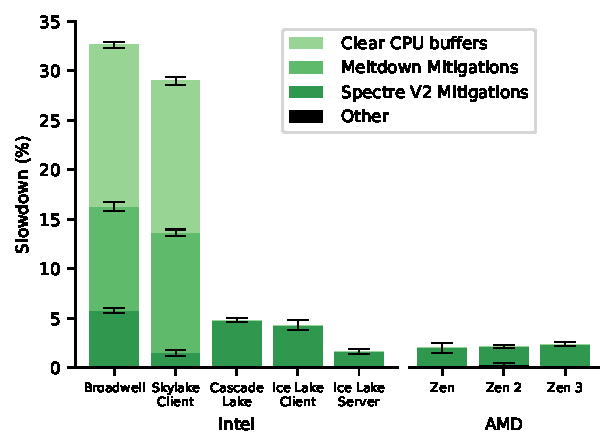
\includegraphics[width=\columnwidth]{plots/lebench.pdf}
    \caption{The overhead of mitigations on the LEBench benchmark suite which stresses the operating system interface.}
    \label{fig:lebench}
\end{figure}


LEBench~\cite{ren:lebench} is a collection of microbenchmarks for measuring specific operating system operations.\footnote{To align with experiments from elsewhere in this thesis, we use the version of the LEBench benchmarks distributed with \sys~\cite{behrens:ward} .}
In this experiment, we track the geometric mean of benchmarks from the suite.
As seen in Figure~\ref{fig:lebench} the overhead has decreased sharply for newer processors:
CPUs which incorporate hardware mitigations (for Intel) or from a vendor whose CPUs were not vulnerable to all attacks in the first place (AMD) exhibit substantially smaller overheads.

Also notable is that only a small number of mitigations are responsible for nearly all of the overheads.
Collectively, all unlisted mitigations caused a fraction of a percent slowdown on Zen 2, but on our other processors had no statistically significant impact at all.

\subsection{Octane 2}
\label{sec:benchmarks:octane-2}

\begin{figure}[t]
    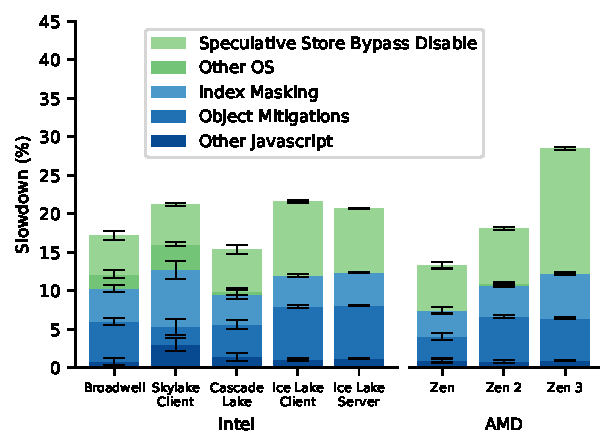
\includegraphics[width=\columnwidth]{plots/octane2.pdf}
    \caption{Slowdown on the Octane 2 browser benchmark caused by JavaScript and operating system level mitigations.}
    \label{fig:octane2}
\end{figure}

Octane 2 is a benchmark for JavaScript performance, which we run from within Firefox.
Figure~\ref{fig:octane2} plots the percent decrease in scores caused by enabling each mitigation in turn.
JavaScript mitigations (Index masking, object mitigations, and ``other JavaScript'') are shown in blue, while operating system controlled mitigations including Speculative Store Bypass Disable (SSBD) and ``other OS'' are shown below them in green.

All JavaScript mitigations are implemented by the JIT engine inserting extra instructions into the generated instruction stream, and are used to prevent different variations of the Spectre V1 attack.
For instance, index masking ensures that speculative accesses to an array do not index past the end of an array.
It does so by placing a conditional move instruction before every array access which checks whether the access is in bounds and overwrites the index with zero otherwise.
This check overall takes very little time but it prevents the CPU from starting to pull the array contents into cache until the array length is known.
Across many millions of array accesses in the Octane 2 benchmark, this ends up causing a non-trivial cost.

Speculative Store Bypass Disable is an OS level mitigation that is disabled by default for most processes, but which Firefox specifically opts into.
It does so to provide stronger sandboxing of JavaScript execution.
Intel has reserved a bit in in the \texttt{ARCH\_CAPABILITIES} model-specific register to indicate that a given processor isn't vulnerable to Speculative Store Bypass and therefore that the associated mitigation is neither needed nor implemented.
However, we do not know of any CPUs for either vendor that set that bit, not even models that came out years after the attack was discovered.

\subsection{Virtual Machine Workloads}
\label{sec:benchmarks:vm}

We measure two different virtual machine workloads relevant to how VMs are used in production.
The performance of running LEBench inside of a KVM virtual machine with and without host mitigations enabled mirrors running a customer application on a cloud provider.
Execution primarily (but not exclusively) stays within the VM so we would expect host mitigations to have limited impact on the performance observed by the guest.
This matches our observations: measured overhead was $\pm 3$\% on all systems, signalling that the mitigations applied by a hypervisor do not have significant impact.
Some runs suggested a slowdown in the range of 1-3\%, but our methodology resulted in too much variability between runs to be confident whether or not that was caused by noise. 
In any case, we were unable to attribute the slowdown to specific mitigations.

Secondly, we measure the overhead of virtual machine exits by running the \textit{smallfile} and \textit{largefile} microbenchmarks from LFS~\cite{rosenblum:lfs} against an emulated disk.
In this workload there are significant numbers of security boundary crossings because every access to the emulated disk requires running code within the hypervisor.
The median overhead was under $2$\%, but once again, we observed high variability between runs.
On many configurations there was no statistically significant difference between running with and without host mitigations at all.

\subsection{PARSEC}
\label{sec:benchmarks:parsec}
As a final experiment we measure the overhead of running the \textit{swaptions}, \textit{facesim}, and \textit{bodytrack} benchmarks from the PARSEC suite.
These were chosen to get good coverage of benchmarks with different working set sizes.
None involve significant numbers of calls into the operating system nor user-level sandboxing, as explored by the previous experiments, which makes them ideal to measure the impact solely of ``always on'' mitigations that the OS applies to running processes.

We were unable to observe any meaningful difference between running with and without the default set of mitigations: total runtime was usually within $\pm0.5$\% for the two configurations, and never differed by more than $2$\%.
This matches prior reports that compute intensive workloads without interactions with the OS do not suffer much from mitigations, and serves as a reminder that slowdowns from transient execution attack mitigations aren't relevant to all workloads.

The one exception is that when we force-enabled mitigations for Speculative Store Bypass, we observed significant overheads which \S\ref{sec:ssb} explores in more detail.

\subsection{Summary}
Each of these benchmarks plots a very different trajectory of mitigation costs.
Workloads that stress the operating system interface have received the most attention, and overheads on LEBench have gone from over 30\% on older Intel CPUs to under 3\% on the latest models from both vendors.
By contrast, JavaScript overhead has been consistently in the range of 15\% to 25\%, with the newest AMD processor we tested paying an even larger cost.
Our compute-intensive benchmark has negligible overhead regardless of the processor.

Preventing Spectre V1 has been a significant goal for computer architecture research, but interestingly software mitigations for it had no measurable impact on LEBench performance.
By contrast, they account for nearly half the overhead on the browser workload.

It is also worth pointing out that all three attacks with significant overhead on new processor are actually quite old.
Spectre V1 and Spectre V2 were the first transient execution attacks discovered (along with Meltdown which was discovered at the same time) while Speculative Store Bypass followed only a matter of months later.
Over the subsequent three years of transient execution attack discoveries, they've all either been quickly resolved in hardware or had a negligible cost to mitigate in software.
This paints an optimistic outlook for the future.

\section{Performance of Individual Mitigations}
\label{s:evolution-eval}

This section explores in more detail the individual mitigations that contributed
to the previously shown end-to-end overheads.
Our aim is to understand why some mitigation costs have gone down while others have not.

For each mitigation, we attempt to isolate the relevant instruction sequence and examine what the cost is on each of our processors.
To achieve precise timings, we rely on the timestamp counter functionality available on x86 and average over one million runs to eliminate noise.

\subsection{Meltdown}

On LEBench, Meltdown accounts for one of the most substantial performance impacts, singlehandedly causing an around 10\% overhead on its own.
On processors vulnerable to Meltdown, production operating systems use page table isolation (PTI) to mitigate it.
This approach adds significant overhead to every user-kernel boundary crossing, because it requires switching the page tables every time via a \texttt{mov} to the \texttt{\%cr3} register.
Among the systems we evaulated, only Broadwell and Skylake are vulnerable to Meltdown.

As seen in Table~\ref{table:meltdown}, on processors vulnerable to Meltdown the cycles required to swap page tables when entering and again on leaving the kernel far exceeds the time for the actual \texttt{syscall} or \texttt{sysret} instruction that triggers the entry/exit.
For syscalls, the Ice Lake Client CPU takes fewer cycles (which will prove a pattern---likely due to its lower base clock speed) and the Cascade Lake model stands out by taking longer than both earlier and later Intel models.

\begin{table}[h]
  \begin{center}
  \begin{tabular}{clccc} 
    \textbf{Vendor} & \textbf{CPU} & \textbf{\texttt{syscall}} & \textbf{\texttt{sysret}}  & \textbf{swap \texttt{cr3}} \\ \hline 
    \multirow{5}{*}{Intel} & Broadwell             & 49 & 40 & 206 \\
                           & Skylake Client        & 42 & 42 & 191 \\
                           & Cascade Lake          & 70 & 43 & 0 \\
                           & Ice Lake Client       & 21 & 29 & 0 \\
                           & Ice Lake Server       & 45 & 32 & 0 \\ \hline
      \multirow{3}{*}{AMD} & Zen                   & 63 & 53 & 0 \\
                           & Zen 2                 & 53 & 46 & 0 \\
                           & Zen 3                 & 83 & 55 & 0 \\ \hline
  \end{tabular}
  \end{center}
  \caption{Average cycles to execute a \texttt{syscall} or \texttt{sysret} instruction, and for vulnerable processors, to swap page tables. }
  \label{table:meltdown}
\end{table}

One other impact of page table isolation is that on very old processors it can cause increased TLB pressure due to much more frequent TLB flushes.
Both Broadwell and Skylake Client, however, support PCIDs which tag page table entries with a process identifier.
This means that on those processors the TLB has to be flushed much less often, and makes TLB impacts marginal compared to the direct cost switching the root page table pointer.

\subsection{Microarchitectural Data Sampling}

The other substantial mitigation on LEBench is clearing CPU buffers, which is required to mitigate Microarchitectural Data Sampling (MDS).
On processors that are vulnerable to MDS, a microcode patch extends the \texttt{verw} instruction to also implement this clearing functionality.
Without the patch the \texttt{verw} only has its old behavior related to segmentation.

Table~\ref{table:verw} shows that the cost of performing this flush is approximately 500 cycles.
This cost is substantial because microarchitectural buffers must be flushed not
just on context switches between processes but also on every kernel-to-user privilege transition.
Recent Intel processors and well as all AMD processors are not vulnerable to MDS.
On these processors the \texttt{verw} has only its legacy segmentation-related behavior and takes only tens of cycles.

\begin{table}[h]
  \begin{center}
  \begin{tabular}{clc}
      \textbf{Vendor} & \textbf{CPU} & \textbf{Clear Cycles} \\ \hline 
      \multirow{5}{*}{Intel} & Broadwell             & 610 \\
                             & Skylake Client        & 518 \\
                             & Cascade Lake          & 458 \\
                             & Ice Lake Client       & 0 \\
                             & Ice Lake Server       & 0 \\ \hline
      \multirow{3}{*}{AMD}   & Zen                   & 0 \\
                             & Zen 2                 & 0 \\
                             & Zen 3                 & 0 \\ \hline
  \end{tabular}
  \end{center}
  \caption{Cycles required to clear microarchitectural buffers using the
    \texttt{verw} instruction. Processors not vulnerable to MDS are listed as
    zero cycles because they do not require any microarchitectural buffers to be cleared before returning to user space. }
  \label{table:verw}
\end{table}

\subsection{Spectre V2}

Spectre V2 involves poisoning the branch target buffer so that an indirect branch in victim code jumps to a Spectre gadget.
Mitigating Spectre V2 is a small but largely consistent drag on LEBench performance across all our processors.

\subsubsection{Indirect Branch Restricted Speculation}

Indirect Branch Restricted Speculation (IBRS) was the first mitigated proposed for Spectre V2 and is enabled by setting a MSR bit which must be repeated on every entry into the kernel.
Newer Intel processors---Cascade Lake and onward---support extended IBRS (eIBRS), which allows the operating system to enable IBRS once at boot time, and have it remain in effect without additional system register writes.

The cycle cost of doing this MSR write on every system call was viewed as unacceptably high, so production operating systems investigated alternative approaches, ultimately settling on retpolines for any processor not supporting eIBRS.

\subsubsection{Retpoline}

Retpolines are the primary software mitigation for Spectre V2 today.
They involve replacing every indirect branch in the kernel with an alternate instruction sequence.
A retpoline sequence has identical behavior to an indirect branch instruction, except that the branch destination (and more importantly any Spectre gadgets) are never jumped to speculatively.

There are a couple variations of retpolines, with slightly different characteristics.
So called ``generic retpolines'' use a code sequence involving a \texttt{call} instruction, a write instruction to replace the saved return address with the jump target, and a \texttt{ret} instruction to cause the processor to speculatively jump back to the call site (due to the return value stack) before correcting to the intended branch target.
This version works on both Intel and AMD processors.

An alternative version ``AMD retpoline'', involves simply doing an \texttt{lfence} followed by a normal indirect branch.
As might be inferred from the name, this variant does not work on Intel: code using it would still be vulnerable to Spectre V2.

\begin{figure}[h]
  \begin{lstlisting}[language={[x86masm]Assembler}]
generic_retpoline:
    call 2f
1:  pause
    lfence
    jmp 1b
2:  mov %r11, (%rsp)
    ret

amd_retpoline:
    lfence
    call *%r11\end{lstlisting}
  \caption{Assembly sequences for the two kinds of retpolines}
  \label{fig:retpoline-samples}
  \end{figure}

Table~\ref{table:retpoline} shows extra cycles of each of these variations across our machines, relative to a baseline of doing an unsafe indirect branch.
One noticeable takeaway is that IBRS adds tens of cycles of overhead to indirect branches except on processors with eIBRS support (Cascade Lake and the two Ice Lake CPUs) where it is inexpensive.
Retpolines however can be as or even more costly.

The AMD processors have different performance executing AMD
retpolines: on the Zen 2 model we measure no overhead compared to a
normal indirect branch, while the other AMD processors they are even
slower than a generic retpoline.

%The main takeaway is consistent with the LEBench results: mitigation costs have remained small but non-trivial across processor generations.




\begin{table}[h]
\begin{center}
\begin{tabular}{ clcccc }
  \textbf{Vendor} & \textbf{CPU} & \textbf{Baseline} & \textbf{IBRS} & \textbf{Generic} & \textbf{AMD} \\ \hline
  \multirow{5}{*}{Intel} & Broadwell           & 16 & +32 & +28 & \tiny{N/A} \\
                         & Skylake Client      & 11 & +15 & +19 & \tiny{N/A} \\
                         & Cascade Lake        & 3 & +0 & +49 & \tiny{N/A} \\
                         & Ice Lake Client     & 5 & +0 & +21 & \tiny{N/A} \\
                         & Ice Lake Server     & 1 & +1 & +50 & \tiny{N/A} \\ \hline
  \multirow{3}{*}{AMD}   & Zen                 & 30 & \tiny{N/A} & +25 & +28 \\
                         & Zen 2               & 3 & +13 & +14 & +0 \\
                         & Zen 3               & 23 & +19 & +13 & +18 \\ \hline
\end{tabular}
\end{center}
\caption{Baseline cycles to perform an indirect branch, and the added cost of doing indirect branches with IBRS enabled, the added cost of an indirect branch via a generic repoline, and via an AMD retpoline.}
\label{table:retpoline}
\end{table}

\subsubsection{Indirect Branch Prediction Barrier (IBPB)}

In addition to preventing indirect branches in the kernel from being
hijacked, it is also important that one user process cannot launch a Spectre V2 attack against another process.
To prevent this attack, on every context switch between processes the operating system runs an Indirect Branch Prediction Barrier to clear the branch target buffer.

We verified across all our processors that executing an IBPB between poisoning the branch target buffer and performing an indirect branch prevents execution from being routed to the attacker-controlled target.
Oddly, however, we noticed that the performance counters report that indirect branches executed after an IBPB result in mispredictions.
We speculate that this behavior is caused by the IBPB setting all entries in the BTB to point to a specific harmless gadget rather than simply clearing them.

Table~\ref{table:ibpb} shows that the cost of an IBPB has generally
declined over time from many thousands of cycles on our Broadwell
server to hundreds of cycles on Cascade Lake and Ice Lake Server.
This improvement is likely related to the fact that older processors implemented IBPB via a microcode patch, whereas newer ones may have some amount of support in hardware.
Our Ice Lake Client processor somewhat bucks the trend of improving performance when compared to the earlier Cascade Lake, but still requires many fewer cycles than Broadwell or Skylake.
AMD processors we tested show a similar improvement across generations.

\begin{table}[h]
    \begin{center}
    \begin{tabular}{ clc }
      \textbf{Vendor} & \textbf{CPU} & \textbf{IBPB cycles} \\ \hline

      \multirow{5}{*}{Intel} & Broadwell         & 5573 \\
                             & Skylake Client    & 4537 \\
                             & Cascade Lake      & 340 \\
                             & Ice Lake Client   & 2455 \\
                             & Ice Lake Server   & 836 \\ \hline
      \multirow{3}{*}{AMD}   & Zen               & 7370 \\
                             & Zen 2             & 1088 \\
                             & Zen 3             & 808 \\ \hline
    \end{tabular}
    \end{center}
    \caption{Cycles to execute an indirect branch speculation barrier. }
    \label{table:ibpb}
\end{table}

\subsubsection{Return Stack Buffer Filling}

When a user process employs generic retpolines to protect itself from Spectre V2, it is counting on the return stack buffer not being tampered with during the code sequence.
Unfortunately, if the operating system triggers a context switch at an inopportune time then this condition might be violated.
Linux uses two approaches to guarantee that user-level retpolines still work despite interrupts potentially happening at any time during execution.

The first is a static analysis pass over the Linux kernel at build time to ensure that the operating system itself doesn't have  unbalanced \texttt{call} and \texttt{ret} pairs anywhere, which incurs no runtime cost at all.
Since any code compiled with the regular toolchains will already have this property, this check is not expected ever to fail.

Secondly, when context switching between different user threads Linux will fill the the return stack buffer with harmless entries.
This is required so that any interrupted retpoline sequence will avoid jumping to any Spectre gadgets---meaning that despite not causing a speculative jump to the intended retpoline landing point, it will still produce safe results.

Table~\ref{table:rsb-fill} shows the cycles required to fill the return stack buffer on each processor.
There is improvement across generations of Intel processors but less of a clear trend across the AMD CPUs.
These changes are likely realized more by improving performance overall
than trying to optimize for return stack buffer filling specifically, but regardless, the cost of these mitigations is relatively minor compared to the total overhead of doing a context switch between processes.

\begin{table}[h]
  \begin{center}
  \begin{tabular}{clc}
      \textbf{Vendor} & \textbf{CPU} & \textbf{RSB Fill Cycles} \\ \hline
      \multirow{5}{*}{Intel} & Broadwell       & 130 \\
                             & Skylake Client  & 130 \\
                             & Cascade Lake    & 120 \\
                             & Ice Lake Client & 40 \\
                             & Ice Lake Server & 69 \\ \hline
      \multirow{3}{*}{AMD}   & Zen             & 114 \\
                             & Zen 2           & 68 \\
                             & Zen 3           & 94 \\ \hline
  \end{tabular}
  \end{center}
  \caption{Cycles to stuff the RSB. }
  \label{table:rsb-fill}
\end{table}

Return stack buffer filling also provides protection against variations of
SpectreRSB, which exploits the return stack buffer itself.
Thus while the overall toggle to enable the functionality is controlled by Linux's \texttt{nospectre\_v2} option, some amount of the overhead attributed to Spectre V2 should probably be accounted to mitigating SpectreRSB instead.

\subsection{Spectre V1}

On the Octane 2 benchmarks, the various Spectre V1 mitigations collectively accounted for a large fraction of the total overhead.
We discuss each of them in more detail.

\subsubsection{lfence}

One mitigation for Spectre V1 is to execute an \texttt{lfence} instruction immediately following each bounds check and \texttt{swapgs} instruction.
This instruction waits until all prior loads have resolved, thereby preventing any subsequent Spectre gadget from executing.
The cost of an \texttt{lfence} varies significantly based on operations in flight.
A simple microbenchmark of running the instruction in a loop shows improvement between successive generations of Intel processors, but AMD's Zen 3 is actually slower than its predecessor.

Table~\ref{table:lfence} shows the cost of executing a single \texttt{lfence} instruction, with the important caveat that the performance of the instruction depends a lot on what other instructions have been executed prior.
We see that all times are roughly of the same scale, with newer processors showing better performance.
The \texttt{lfence} does more work on AMD than on Intel (as evidenced by the AMD retpoline sequence described earlier) so the numbers are not directly comparable across vendors.

\begin{table}[h]
  \begin{center}
  \begin{tabular}{ clc }
    \textbf{Vendor} & \textbf{CPU} & \textbf{lfence cycles} \\ \hline
    \multirow{5}{*}{Intel} & Broadwell        & 28 \\
                           & Skylake Client   & 20 \\
                           & Cascade Lake     & 15 \\
                           & Ice Lake Client  & 8 \\
                           & Ice Lake Server  & 13  \\ \hline
    \multirow{3}{*}{AMD}   & Zen              & 48 \\
                           & Zen 2            & 4 \\
                           & Zen 3            & 30 \\ \hline
  \end{tabular}
  \end{center}
  \caption{Cycles to execute a single lfence instruction on each machine.
    In real applications, the cost will heavily depend on the other loads in flight. }
  \label{table:lfence}
\end{table}

\subsubsection{Index Masking}

Instead of preventing speculation past bounds checks, an alternative mitigation is to force the array index to zero for any out of bounds access.
SpiderMonkey (the JavaScript engine used by Firefox) uses this
strategy: before every array indexing operation it inserts a
\texttt{cmov} instruction that overwrites the array index with zero if it would be past the end of the array.
Unlike in many compiled languages, JavaScript always knows the lengths of arrays so this mitigation can be applied automatically to the generated assembly.
On the committed execution path the conditional move will always be a no-op (because as a safe language JavaScript always does bounds checks), but in the speculative case it blocks execution until the array length has resolved.
Our measurements of the Octane 2 benchmark suite indicate this approach incurs an approximately 4\% performance overhead.

\subsubsection{Object Mitigations}

Since JavaScript is dynamically typed, the compiler must insert many runtime checks on the types of variables.
This presents another possible avenue for Spectre V1 attacks, because mis-speculating an object's type can cause its fields to be misinterpreted, potentially resulting in out of bounds memory reads.
The mitigation is similar to index masking: object guards insert a conditional move that zeros out the object pointer if the check check fails.
This mitigation incurs an overhead on Octane 2 on the order of 6\%.

\subsection{Speculative Store Bypass}
\label{sec:ssb}

\begin{figure}[h]
  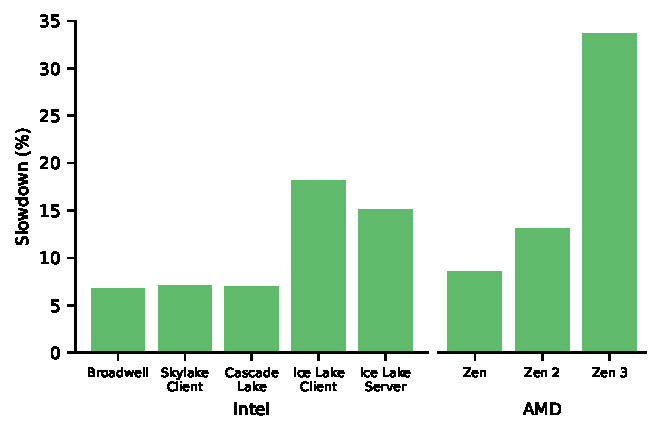
\includegraphics[width=\columnwidth]{plots/ssbd.pdf}
  \caption{The slowdown caused by Speculative Store Bypass Disable on three benchmarks from the PARSEC suite.}
  \label{fig:ssbd}
\end{figure}

Speculative Store Bypass, originally called Spectre V4, exploits the processor's store-to-load forwarding to enable an attacker to learn the contents of recently written memory locations.
The only available defense against the attack is to enable a processor mode called Speculative Store Bypass Disable (SSBD) that blocks this forwarding.
A downside is that this can come at substantial cost, even when normal non-malicious code is being run.

The compromise reached by the Linux developers was to enable SSBD only for processes which opted into it via its \texttt{prctl} or \texttt{seccomp} interfaces.
To see the full impact of this mitigation if enabled all the time, we measured the slowdown it causes to the swaptions benchmark from PARSEC.
Figure~\ref{fig:ssbd} shows that the slowdown can be as much as 34\%,
and is trending worse over time.
It isn't entirely clear why this would be the case, but it may be related to newer processors have a more complete SSBD implementation compared to what was possible via microcode patches.
These overheads are especially considerable given that the combined
impact of all default mitigations for this benchmarks is well under one percent (\S\ref{sec:benchmarks:parsec}).

\subsection{L1 Terminal Fault}
One other attack worth mentioning is L1 Terminal Fault, which can leak the entire contents of the L1 cache when page tables contain PTEs with certain bit patterns.

Linux avoids ever creating such PTEs (which can be done with essentially no overhead).
However, the problem is more severe when virtual machines are involved because an untrusted guest operating system could insert such specially crafted PTEs into its own page table.
Doing so would enable it to learn L1 cache contents lingering from memory accesses done by the host, and so the necessary mitigation on vulnerable processors is for the host to flush the L1 cache prior to entering a guest virtual machine.

Our benchmarking of virtual machine workloads did not show any measurable impact from enabling this mitigation and it has also been patched on newer processors, so the relevance should be minimal going forward.

\subsection{Other attacks}

The attacks discussed so far are hardly the only transient execution attacks discovered.
Many others like FPU Register Bypass, System Register Read, and so forth have commanded significant time and attention for computer architects, operating system developers, and security researchers.
However, the cost they incur on workloads today seems to be minimal, so we skip evaluating them individually.


\begin{figure}[h]
\begin{lstlisting}
void victim_target() {
  int c = 12345 / 6789;
}
void nop_target() { /* do nothing */ }

void(*target)();

void test() {
  // configure performance counter to measure
  // whether the divider is active
  configure_pmc(ARITH_DIVIDER_ACTIVE);

  // train the branch target buffer
  target = victim_target;
  for (int i = 0; i < 1024; i++)
    divide_happened();

  // potentially overwrite the entry
  ...

  // measure whether the trained entry is jumped
  // to speculatively
  target = nop_target;
  if (divide_happened())
    printf("victim_target ran speculatively!");
}

bool divide_happened() {
  // fill branch history buffer
  for (int i = 0; i < 128; i++) {}

  // flush branch target from cache
  clflush(target);

  // read performance counter
  int start = rdpmc();

  // perform the indirect branch
  (*target)();

  // see whether performance counter changed
  return rdpmc() > start;
}\end{lstlisting}
\caption{Sketch of our approach. The \texttt{test} function prints whether it was able to poison the branch target buffer to route speculative execution to \texttt{victim\_target}.}
\label{fig:spectre2-sample}
\end{figure}

\begin{table*}[ht]
    \begin{center}
    \begin{tabular}{ clccccc } 
      && \multicolumn{3}{r}{\textbf{With intervening system call}} & \multicolumn{2}{c}{\textbf{No system call}} \\
      \textbf{Vendor} & \textbf{CPU} & u$\rightarrow$k & u$\rightarrow$u & k$\rightarrow$k & u$\rightarrow$u & k$\rightarrow$k \\ \hline 
      \multirow{5}{*}{Intel} & Broadwell           & \checkmark & \checkmark & \checkmark & \checkmark & \checkmark \\
                             & Skylake Client    & \checkmark & \checkmark & \checkmark & \checkmark & \checkmark \\
                             & Cascade Lake        &            & \checkmark & \checkmark & \checkmark & \checkmark \\ 
                             & Ice Lake Client   &            & \checkmark & \checkmark & \checkmark & \checkmark \\ 
                             & Ice Lake Server   &            & \checkmark & \checkmark & \checkmark & \checkmark \\ \hline
      \multirow{3}{*}{AMD}   & Zen             & \textcolor{red}{X} & \textcolor{red}{X} & \textcolor{red}{X} & \textcolor{red}{X} & \textcolor{red}{X} \\
                             & Zen 2           & \checkmark & \checkmark & \checkmark & \checkmark & \checkmark \\
                             & Zen 3         &  &  &  &  & \\ \hline
    \end{tabular}
    \end{center}
    \caption{ Whether the processor will speculatively execute an indirect branch in the given configuration when IBRS is disabled.
              A checkmark in column X$\rightarrow$Y indicates that training the branch target buffer in mode X is able
              to control the target of a subsequent victim indirect branch in mode Y, either with or without an intervening \texttt{syscall} and/or \texttt{sysret} instruction between them.}
    \label{table:btb-no-ibrs}
  \end{table*}
  
  \begin{table*}[ht]
    \begin{center}
    \begin{tabular}{ clccccc } 
      && \multicolumn{3}{c}{\textbf{With intervening system call}} & \multicolumn{2}{c}{\textbf{No system call}} \\
      \textbf{Vendor} & \textbf{CPU} & u$\rightarrow$k & u$\rightarrow$u & k$\rightarrow$k & u$\rightarrow$u & k$\rightarrow$k \\ \hline 
      \multirow{5}{*}{Intel} & Broadwell           & & & & & \\
                             & Skylake Client   & & & & & \\
                             & Cascade Lake      &            & \checkmark & \checkmark & \checkmark & \checkmark \\ 
                             & Ice Lake Client   &            & \checkmark &             & \checkmark &  \\ 
                             & Ice Lake Server   &            & \checkmark & \checkmark  & \checkmark & \checkmark \\ \hline
      \multirow{3}{*}{AMD}   & Zen            & \tiny{N/A} & \tiny{N/A} & \tiny{N/A} & \tiny{N/A} & \tiny{N/A} \\
                             & Zen 2           & & & & & \\
                             & Zen 3         & & & & & \\ \hline
    \end{tabular}
    \end{center}
    \caption{ Same as Table~\ref{table:btb-no-ibrs} but with IBRS \textit{enabled}.
              IBRS always prevents problematic cases like u$\rightarrow$k, but on many processors blocks all speculation including predicting the target of userspace indirect branches based on prior branches done by the same process (u$\rightarrow$u).
    }
    \label{table:btb-ibrs}
  \end{table*}
  
\section{Analysis of Hardware Spectre V2 Mitigations}
\label{s:analysis}

For nearly all the attacks we've looked at so far, either the mitigation approach has remained the same across all the processor generations we've studied, or it has gone from an expensive software mitigation to a hardware fix with no measurable cost at all.
Spectre V2 notably does not follow this trajectory.
It has an array of hardware and software mitigations, yet remains a non-trivial expense on every CPU we've tested.
In this section we attempt to understand under which conditions the
Branch Target Buffer is used to speculatively execute instructions and when not.


\subsection{Measuring Speculation}

To understand when CPUs speculatively execute instructions, we need a
method to determine what instructions are being speculatively executed
by the CPU.  Bölük~\cite{speculating-x86} describes a technique using
performance counters to determine whether a processor starts
speculatively executing at a given address, which we adopt to probe
the behavior of the Branch Target Buffer, as we describe next.

% \fk{is the point of this paragraph to say that every processor has
%   performance counters for division operations, while not all
%   processors have dedicated performance counters for mispredicted
%   indirect branches? if so we should just  say that}
The performance counters are specific to an individual generation of CPU and provide detailed information about microarchitectural events.
All our processors have a performance counter to measure the number of cycles that the divider is active, and some also have a dedicated performance counter to indicate the number of mispredicted indirect branches.
By reading one of these counters before and after a block of instructions, we can tell whether executing that code triggered any of the relevant operations.

Figure~\ref{fig:spectre2-sample} sketches out how we use this method to know whether code at a specific target location was executed speculatively.
We execute indirect branches that may potentially be mispredicted as targeting a specially constructed landing pad, and see whether we measure any use of the divider corresponding to executing instructions at landing pad.
Care has to be taken to ensure no divide instructions are executed by the committed execution trace.

Interestingly, we sometimes observed mispredicted indirect branches without any divide instructions being performed, which we interpret as the processor speculatively executing instructions at a different location than the one we attempted to poison the branch target buffer with.
For this reason, we focus on the performance counter for cycles with the divider active even when both are available.

% This in turn tells us tell whether which entries are in the branch target buffer.

% Directly using that counter is more precise than counting the number of divide operations.

Prior work discovered that for a Spectre V2 attack, only some bits of the virtual and physical addresses have to match between the victim and attacker.
However, to maximize the chance of success, we ensure all 64 bits match by sharing the same page of memory between the victim and attacker.

\subsection{Results}

Tables~\ref{table:btb-no-ibrs} and \ref{table:btb-ibrs} show the results produced using this methodology.
The columns indicate the mode that the attacker and victim run in
respectively (e.g., user$\rightarrow$kernel is the classic
configuration of a user-space attacker trying to misdirect a victim running in kernel space).
We also indicate the presence of an intervening \texttt{syscall} instruction.

Not shown in that figure, we also attempted to run the attacker in kernel mode and the victim in user mode.
This is not reflective of a real world attack scenario, but it revealed that the same attacks processors vulnerable to the user$\rightarrow$kernel version were vulnerable to a kernel$\rightarrow$user attack.

One final note is that we did not manage to poison the branch target buffer at all on our Zen 2 processor.
We suspect this isn't because it is immune to the attack, but rather due to some change to the Branch History Buffer (used to compute the index for the branch target buffer) or another implementation detail that experiments did not account for.

\subsubsection{Indirect Branch Restricted Speculation}

Recall that the original version of Indirect Branch Restricted Speculation (IBRS) was the first mitigation proposed for Spectre V2 but is not used by default on any production operating system because it requires an expensive write to a model-specific register on every entry into the kernel.

According to Intel documentation, this mitigation prevents indirect branches executed from less privileged modes from impacting the predicted destination of indirect branches in more privileged modes.
We experimentally validated this claim by poisoning the branch target buffer and then seeing whether the processor would speculatively jump to the programmed branch destination.
Our measurements indicated that toggling this mitigation caused the
user space code to be unable to redirect kernel execution.
However, subsequent experiments (replicated in
Table~\ref{table:btb-ibrs}) revealed that IBRS was disabling all
indirect branch prediction both in user space and kernel space.
Not having this prediction even for user processes incurs a high performance cost.

\subsubsection{Enhanced IBRS (eIBRS)}

Enhanced IBRS provides the same guarantees as the original IBRS but doesn't require an MSR write on every kernel entry.
Given the lackluster performance of IBRS compared to retpolines, that may not seem promising, but the presence of this feature signals more serious mitigations built into the hardware.
In particular, eIBRS does not disrupt indirect branch prediction at the same privilege level.
When it is available, Linux by default uses eIBRS instead of retpolines.

As seen in Table~\ref{table:btb-ibrs}, Cascade Lake and the two Ice Lake
processors (the microarchictures that support eIBRS) both do indirect branch prediction only based on prior indirect branches executed in the same privilege mode.
We speculate this is achieved by using a branch target buffer that is either partitioned or tagged using a bit indicating the current privilege mode.

When running with eIBRS enabled, we have observed that kernel entries (caused by page faults, the \texttt{syscall} instruction, etc.) having bimodal performance.
Most times they take a similar number of cycles (on the order of 70 cycles), but one in every 8 to 20 or so entries they take an additional 210 cycles.
On the same processor, when running without eIBRS the time is always 70 cycles.

We have been unable to fully determine what is causing this behavior, but a few patterns have emerged.
Under some conditions, the slow system calls will happen exactly every eight times, meanwhile at other times the processor will go long stretches without any slow syscalls.
Additionally, we have sometimes observed behavior consistent with the branch target buffer being flushed only during slow kernel entries: poisoning the branch target buffer in the kernel prior to a system call causes misprediction of subsequent indirect branches in kernel mode only if the intervening kernel entry was fast.
Monitoring performance counters reveal that slow system calls involve both executing more micro ops and more cycles spent stalling, but do not provide a clear hint of what those additional micro ops are doing.

\subsection{Takeaways}
The original IBRS design not only added substantial overhead to every kernel entry, it also blocked indirect branch speculation everywhere.
eIBRS improves on this by seemingly partitioning or tagging the branch target buffer based on the CPU privilege mode.

Partitioning / tagging the branch target buffer however is not a complete mitigation for Spectre V2.
User processes still need their own defenses and even within the kernel indirect branches executed by the operating system could be used to mistrain the branch target buffer to misdirect subsequent operating system indirect branches.

We suspect that the designers of eIBRS may have been aware of this risk and taken precautions against it.
The documentation for eIBRS doesn't make any promises, but the slow kernel entries suggest that additional work is happening in connection with the feature.

\section{Discussion}
\label{s:discussion}

We present some thoughts for computer architects and
operating systems developers that can address the lingering slowdowns from transient execution attacks.

\subsection{Hardware mitigations for Spectre V1}

One takeaway from the previous sections is the continued impact of Spectre V1.
There are no hardware mitigations available for the attack in high performance commercial CPUs.
And yet, despite being among the first transient execution attacks discovered, it still presents a significant---and largely unchanging---overhead when mitigated in software.

Because Spectre V1 mitigations are specifically applied by JIT engines doing code generation, they also may present a unique opportunity for computer architects.
The JIT annotates each vulnerable gadget with a leading \texttt{cmov} instruction.
This pattern of a conditional move followed by a load instruction could be detected by hardware to trigger special handling.

Even if this approach proves unworkable, that doesn't rule out hardware acceleration for Spectre V1 mitigations.
JIT engines generate code on the fly based on the processor they are running on, which means that unlike native applications, the author of a given JavaScript application doesn't need to be involved in porting/recompiling it to leverage a new ISA extension.
And since current web browsers generally receive new updates on a six
week release cycle, any new hardware could be leveraged quickly.

\subsection{Speculative Store Bypass}

Speculative Store Bypass Disable was initially implemented in microcode, and while we cannot tell whether more recent CPUs include actual hardware changes as well, the performance overhead hasn't improved.
This attack in particular also emphasizes the need to look at the performance impacts of transient execution attacks across representative workloads.
Despite being disabled by default, Speculative Store Bypass Disable incurs a substantial overhead on JavaScript execution in web browsers---one of the most common workloads run by end-users.

Intel's inclusion of a hardware capability to detect whether a
processor is vulnerable to Speculative Store Bypass (without a way to toggle it) strongly
suggests that they believe future hardware will be able to prevent
the attack with negligible overhead.

\subsection{Hypertheading safety}

The discovery of more and more transient execution attacks has eroded trust that CPUs are capable of fully preventing information leaks between concurrently running tasks scheduled on hyperthread pairs.
This is particularly worrisome given that both many of the existing transient execution attacks work in this setting, and that there are a substantial number of other microarchitectural components that are shared between hyperthreads, which could also present side channels.

Linux by default considers this attack vector not worth worrying about, but a heavy-handed approach that's been adopted by certain cloud providers has been to entirely disable hyperthreading when running client virtual machines.
This approach comes at a high cost because the CPU is no longer able to benefit
from the increased utilization that hyperthreading allows~\cite{intelht}.

There is however another option that operating system developers could pursue.
Since it is safe to simultaneously run two mutually trusting processes
on hyperthread pairs, a more sophisticated scheduling policy could
ensure that only processes that are safe to collocate
are assigned to adjacent logical processors.
One complexity with this strategy is protecting the kernel from snooping by a process running on one hyperthread pair while the other hyperthread is executing a system call.


\chapter{Ward}
\label{ch:ward}

%\section{Introduction}

% Over the last two years, transient execution has emerged as a
% powerful new side-channel attack technique.  Vulnerabilities have
% proliferated~\cite{sok:transient,hill:survey}, with examples now including Meltdown~\cite{lipp:meltdown},
% Spectre~\cite{kocher:spectre}, L1 Terminal Fault~\cite{bulck:foreshadow}, RIDL~\cite{schaik:ridl},
% Fallout~\cite{canella:fallout}, ZombieLoad~\cite{schwarz:zombieload},
% CrossTalk~\cite{ragab:crosstalk}, and SGAxe~\cite{sgaxe}.  In contrast
% with conventional timing-based side-channel attacks~\cite{kocher:timing},
% where the victim must access its data in a specific pattern in order
% to leak it, transient execution attacks are more serious because they
% often allow an attacker to precisely control which memory locations are
% leaked, including memory that might not be accessed on the committed
% execution path.  This is of particular concern to OS kernels, which have
% access to all of physical memory, and therefore could leak data from any
% process through transient execution bugs.  In a public cloud,
% where it is common for mutually distrustful tenants to share
% a single machine~\cite{borg, cpi2}, the threat of transient execution
% is especially concerning.

% A key challenge in addressing transient execution attacks lies in
% minimizing the performance overheads.  CPU and OS designers have
% implemented a range of mitigations to defeat transient execution
% attacks, including state flushing, selectively preventing speculative
% execution, and removing observation channels~\cite{sok:transient}.
% These mitigations impose performance overheads (see
% \autoref{s:motivation}): some of the mitigations must be applied at
% each privilege mode transition (e.g., system call entry and exit), and
% some must be applied to all running code (e.g., retpolines for all
% indirect jumps).  In some cases, they are so expensive that OS vendors
% have decided to leave them disabled by default~\cite{apple_support,
%   microsoft_support}.  Recent processor designs have also incorporated
% mitigations into hardware, which also reduces performance compared to
% earlier processor designs that do not perform such hardware
% mitigations.

%Linux has considered offering
%an option to flush the entire L1 cache on context switch, to protect
%against future transient execution attacks~\cite{linux:vuln,phoronix:5.8}.

% For example,
% microarchitectural data sampling (MDS) vulnurabilities like RIDL and
% Fallout cannot be fully mitigated without turning off hyperthreading,
% reducing overall CPU performance by around 33\%.

To address the severe performance overhead associated with OS level mitigations on older processors, we propose a new hardware/software contract, called the \emph{unmapped speculation contract}, or \contract{} for short.
\contract{} allows the OS kernel
to significantly reduce the overhead of mitigating a particular subset
of transient execution attacks---namely, those that leak arbitrary
memory contents.  The \contract{} says that physical memory that is
unmapped (i.e., physical memory that has no virtual address) cannot
be accessed speculatively.  The
benefit of \contract is two-fold.  From the OS designer perspective,
it provides bounds on what data can be leaked through transient execution,
and, as we show in the rest of this paper, can significantly reduce the
cost of mitigations.  From the hardware designer perspective, \contract
allows the CPU to keep many of the current speculative execution
optimizations and their associated performance benefits.  Most
processor architectures already adhere to \contract; AMD
states that ``AMD processors are designed to not speculate into memory
that is not valid in the current virtual address memory range defined
by the software defined page tables''~\cite[pg. 2]{amd:speculation},
and Intel issued hardware and microcode fixes for bugs that violate
\contract~\cite{intel:meltdown, intel:l1tf}.

To demonstrate the benefits of the unmapped speculation contract,
this thesis presents \sys{}, a novel kernel architecture that uses
selective kernel memory mapping to avoid the costs of transient execution
mitigations.  \sys{} maintains separate kernel memory mappings for each
process, and ensures that the memory mapped in the kernel of a process
does not contain any data that must be kept secret from that process.
As a result, privilege mode switches (e.g., system call entry and exit)
no longer need to employ expensive mitigations, since there are no
secrets that could be leaked by transient execution.  When the \sys{}
kernel must perform operations that require access to unmapped parts
of kernel memory, such as opening a shared file or context-switching
between processes, it explicitly changes kernel memory mappings, and
invokes the same mitigation techniques used by the Linux kernel today.

A key challenge in the \sys design lies in re-architecting the kernel
and its data structures to allow for per-process views of the
kernel address space.  For example, a typical \texttt{proc} structure in
the kernel contains sensitive fields, such as the saved registers of that
process, which should not be leaked to other processes.  At the same time,
every process must be able to invoke the scheduler, which in turn may
need to traverse the list of \texttt{proc} structures on the run queue.
We present several techniques to partition the kernel:
transparent switching of kernel address spaces when accessing sensitive
pages through page faults; using temporary mappings to access unmapped
physical pages; splitting data structures into public and private
parts; etc.

To evaluate the \sys design, we applied it to the sv6 research
kernel~\cite{clements:sc} running on x86 processors.  The sv6 kernel
is a monolithic OS kernel written in C/C++, providing a POSIX
interface similar to (but far less sophisticated than) Linux.  The
simplicity of sv6 allowed us to quickly experiment with and iterate on
\sys's design, since some aspects of \sys's design require global
changes to the entire kernel.  Since sv6 is a monolithic kernel,
our prototype was able to tackle hard problems brought up by kernel
services such as a file system and a POSIX virtual memory system.

We evaluate the performance of our \sys prototype using
\bench~\cite{lebench}, which represents the most important system calls
for a range of application workloads: Spark, Redis, PostgreSQL,
Chromium, and building the Linux kernel.  \bench allows us to precisely
measure the impact of mitigations on system calls that matter
for applications.
% The most recent Intel CPUs (such as Cascade Lake)
% include hardware mitigations that cannot be fully disabled; however, some of
% these mitigations are not needed in \sys.  To avoid the performance
% overhead of such unnecessary mitigations, we run experiments on
% the previous generation of Intel CPUs (Skylake).
%\autoref{s:motivation} discusses these hardware mitigation overheads in
%more detail.

\sys can run the \bench microbenchmarks with small performance
overheads compared to a kernel without mitigations.  For 18 out of
the 30 \bench microbenchmarks, \sys's performance is within 5\% of the
benchmark's performance without any mitigations (but at the cost of some
extra memory overhead).  In the worst case, the overhead is 4.3$\times$
(context switching between processes, where mitigations are unavoidable).
In contrast, standard mitigations incur a median overhead of 19\%, and
a worst case of nearly 7$\times$.  To confirm that \bench results translate
into application performance improvements, we measured the performance
of \texttt{git status}, which incurs 11.2\% overhead in \sys, compared
to 24.6\% with standard mitigations.

%We also report the results of
%a qualitative analysis of known transient execution vulnerabilities,
%which demonstrates that \sys's use of the unmapped speculation contract
%is able to handle all of them on recent x86 hardware and microcode.

%% The performance and security results for the \sys prototype suggest that
%% the \sys approach is a promising one for mitigating the performance overheads
%% of transient execution vulnerabilities.  \sys's design highlights a
%% number of important lessons in re-architecting the kernel to partition
%% the kernel memory across per-process kernel address spaces, which is
%% needed to take advantage of the unmapped speculation contract.  We hope
%% that these lessons will be valuable in re-architecting production kernels,
%% such as Linux, to achieve similar performance gains on real applications.

One of the limitations of \contract{} is that it does not cover all
possible transient execution attacks.  In particular, attacks where
the sensitive information is already present in the architectural or
microarchitectural state of the CPU are not covered by \contract{}.
For instance, the Spectre v3a attack can leak the sensitive contents of
a system register (MSR), instead of leaking sensitive data from memory.
\contract{} does not cover sensitive data that is stored outside of
memory, and \sys applies other mitigations (e.g., as in Linux) to address
those attacks.

%% Another limitation of our evaluation is that we cannot
%% selectively control hardware mitigations in the most recent Intel CPUs,
%% which forces us to use an older processor design for most experiments.

\section{Motivation}
\label{s:motivation}

\begin{figure*}[t]
  \begin{center}
    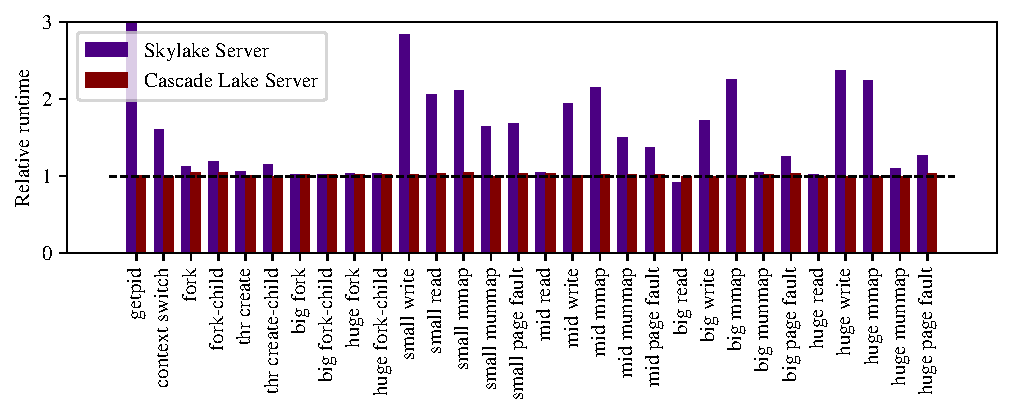
\includegraphics[width=\textwidth]{results/bhw2_bhw3_overhead}
  \end{center}
\vspace{-\baselineskip}
\caption{Linux slowdown due to mitigations on \bench, for two generations of Intel CPUs: Broadwell and Cascade Lake.}
\label{fig:linuxslowdown}
\end{figure*}

% \begin{figure*}[t]
%   \begin{center}
%     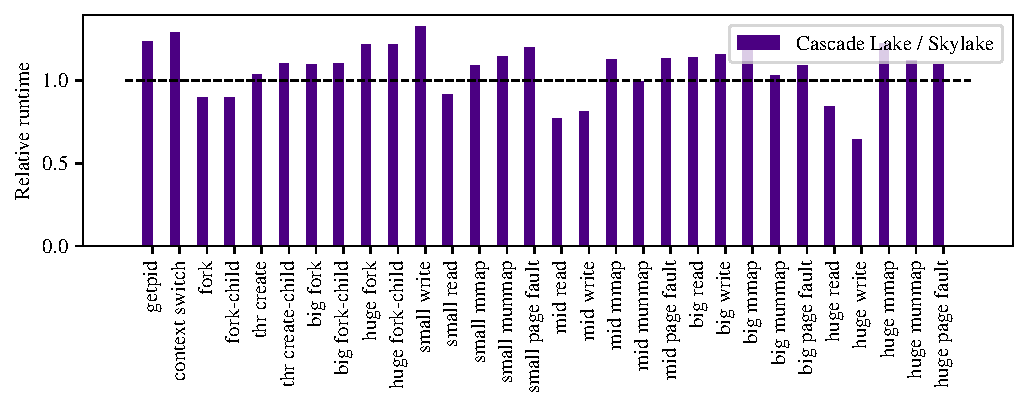
\includegraphics{results/cascade_lake_regression}
%   \end{center}
% \vspace{-\baselineskip}
% \caption{Performance regression on the newer Cascade Lake CPU, compared to the older Broadwell CPU,
%   for \bench on Linux, with all software-controllable mitigations disabled.}
% \label{fig:regression}
% \end{figure*}

Transient execution mitigations harm kernel performance in two
ways. First, they place overhead on code execution by disabling
speculation.  For example, the Linux Kernel uses a retpoline patch to
mitigate Spectre V2, which replaces each indirect branch with a
sequence of instructions that prevent the CPU from performing branch
target speculation~\cite{intel:retpoline}. Second, these mitigations
increase the privilege mode switching cost incurred during each system
call: upon entry into the kernel, they either flush microarchitectural
state or reconfigure protection mechanisms.  For example,
KPTI~\cite{gruss:kaiser,linux:kpti} switches to a separate page table
before executing kernel code to prevent Meltdown
attacks~\cite{lipp:meltdown}.  Workloads
that are system call intensive (e.g., web servers, version control
systems, etc.) are impacted by this type of overhead, while non-kernel
intensive workloads see little performance impact~\cite{gruss:kaiser}.

Collectively, these and other mitigations can result in large
slowdowns. To better understand this problem, we run
\bench~\cite{lebench}, a microbenchmark suite of system calls
that impact application
performance the most.  We evaluate the Linux kernel (version 5.6.13),
comparing two configurations: one where all mitigations are disabled
and one where all are enabled. Figure~\ref{fig:linuxslowdown} shows
the relative slowdown between the two configurations for 13 kernel
operations of \bench that don't involve networking (i.e., without
\texttt{send}, \texttt{recv}, \texttt{epoll}).  There are two sets of
bars, representing two generations of Intel CPUs: the older Broadwell,
and the newer Cascade Lake.  On the older Broadwell CPUs,
system calls that perform the least kernel work are impacted the most
(e.g., \texttt{getpid()}), but a wide range of operations are impacted
significantly (25\%-100\% slowdowns). These observations are similar
to those made by Ren et. al.; they find that KPTI and Spectre V2
mitigations are the root cause of slowdowns in the Linux
Kernel over the last two years~\cite{lebench}.

% The newer Cascade Lake CPUs exhibit lower relative overheads, partly
% because the processors include hardware mitigations for some of the
% transient execution vulnerabilities.  However, these lower overheads
% are also in part due to the newer Cascade Lake CPUs being \emph{slower}
% in the baseline case when software-controllable mitigations are disabled.
% Figure~\ref{fig:regression} shows the performance of the microbenchmark
% on Cascade Lake (Intel Xeon Silver 4210R) relative to the earlier
% Broadwell CPU (Intel Xeon E5-2640 v4).  Our experiment uses CPUs
% with identical clocks (2.4~GHz), and nearly identical other hardware
% (Dell PowerEdge T430 vs. T440), which allows the comparison to be
% meaningful.  The results demonstrate that, although the new CPU is
% faster at some microbenchmarks, it is slower for many others: e.g.,
% context-switching is about 20\% slower.  Although it is impossible for us to
% separate slowdowns due to mitigations from speedups due to architectural
% improvements, the results suggest that the overheads of mitigations implemented
% in hardware (e.g., for Meltdown, L1TF, or MDS) could still be significant.
% \footnote{One indication that this regression may be related to hardware
%   mitigations is that measured branch mispredictions are around 40\% higher on
%   LEBench.}

%\fk{table 11 in ~\cite{sok:transient} claims the overhead of KPTI is
%  small, < 3\%}

%Avoiding these overheads normally requires making compromises to
%security; disabling any one of them would leave the kernel vulnerable
%to a transient execution attack.
%Our goal, instead, is to apply these
%mitigations only when they are needed to protect data that should be
%kept secret from the running process.
%We now describe our approach to
%restructuring the kernel so it can achieve this goal.

\section{Goals}

% This chapter focuses on reducing the overhead of software mitigations, 
% and experimentally measures their effect on the
% previous generations of CPUs predating the discovery , where we can avoid mitigations altogether.
% We hope that \sys's design can allow processor designers to regain some
% of the absolute performance lost due to hardware mitigation costs.

% Our threat model targets scenarios where the adversary
% and the victim are both running code on the same computer.  This might
% arise either in a server setting, where both are running on a cloud
% computing platform, or in a client device, where the adversary code is
% a malicious application or web site.

% Canella et al.~\cite{sok:transient} discuss transient execution attacks
% in detail, but the salient points of the attack boil down to four steps.
% First, the processor speculatively executes some code, which accesses
% sensitive data that the victim wants to keep secret.  Second, during the
% speculative execution, the processor updates microarchitectural state
% in a way that depends on the sensitive data (e.g., bringing in cache
% lines into a shared L3 cache whose addresses depend on the sensitive
% data).  Third, the processor aborts the speculative execution, but does
% not fully roll back all of its side effects (e.g., changes to the L3
% cache), because doing so would be prohibitively expensive in hardware.
% Fourth, the adversary observes these side effects (e.g., using timing
% measurements), which allows the adversary to infer the sensitive data.

OS kernels make a particularly good target for transient execution attacks.
First, an adversary can cause the kernel to speculatively execute code that
leads to leakage of sensitive data. Even though the adversary cannot
inject their own code to execute in the kernel, the adversary can often
have significant influence on what existing kernel code gets executed in
speculative execution, by specifying particular system call arguments or
setting up micro-architectural CPU state such as the branch predictor.
Secondly, an OS kernel has access to all of the state
on the computer. This means that an adversary running in one process
can trick the kernel into leaking state from any other process on the
same computer.

Current OS kernel designs, such as Linux, have two approaches for
mitigating transient execution attacks.  The first approach is to make
sure that the CPU does not speculatively execute any code that could
end up accessing sensitive data.  This approach includes techniques like
retpolines and other speculation barriers.  The second approach is to
make sure that sensitive data is flushed from microarchitectural state,
such as flushing CPU caches and buffers when returning from a system
call or when context-switching between processes.  Both incur significant
performance overheads.

\sys's goal is to reduce the performance cost of mitigations for transient
execution attacks.  In principle, \sys's techniques can reduce not only
the cost of software mitigations, but also allow processor designers
to avoid mitigations in hardware.  Practically, however, \sys 
is most applicable to older Intel processors, which incur the largest
costs on OS-level mitigations.

Transient execution attacks can leak data across many protection domain
boundaries, including leaking secrets from the kernel to an adversary's
process, or leaking secrets from one process to a different process,
or even leaking secrets within a single process that implements its
own internal protection domains.  Much like in the Linux kernel, the
focus of \sys is on preventing leakage between processes, as well as
preventing leakage from the kernel to a process.  \sys's approach to
preventing cross-process leakage is the same as Linux (flushing state),
but \sys has a novel approach for efficiently preventing kernel-to-process
leakage of memory contents, as we describe in the next section.

Although \sys addresses all known transient execution attacks, the focus
here is on attacks that allow the adversary to leak the contents
of arbitrary memory, which is especially important in an OS kernel.
\sys handles other transient execution attacks, such as leaking the
contents of sensitive data already present in the CPU (e.g., x86 MSRs),
in the same way as Linux does.

Attacks that do not leverage transient execution to leak data are also
out of scope, since they are orthogonal to the key
challenge of transient execution leakage.  In particular, we do not
consider attacks that leverage physical side channels (such
as Rowhammer or RAMbleed), cache side channels (such as cache timing
attacks), interrupt side channels, power side channels, etc.

\section{Approach: Unmapped speculation contract}
\label{s:ward-approach}

\sys's design for mitigating transient execution attacks relies
on page tables.  Specifically, if a page of physical
memory is not referenced by any entry in the current page table or
TLB, speculative execution cannot access any sensitive data stored in
that page, because the page doesn't have a virtual address to access
it by.

% Processors typically do
% not speculate on the physical address bits in page table entries, and as a result, the
% lack of a page table entry serves as a barrier to speculative execution.

A contribution of this thesis lies in articulating a hardware/software
contract---which we call the \emph{unmapped speculation contract}---that
captures the above intuition.  The contract aims to provide a strong
foundation for keeping data confidential, which is typically stated as
non-interference.  Non-interference can be thought of by considering
two system states, $s$ and $s'$, that differ only in sensitive data,
which should not be observable by an adversary.  A system ensures
non-interference if an adversary cannot observe any differences in how
the system executes starting from either $s$ or $s'$.

\paragraph{Single-core USC.} To formally state the unmapped speculation contract, we start with a
single-core definition.  We use $A(\cdot)$ to refer to the state of
the CPU, including all architectural and micro-architectural state,
but excluding the contents of memory, and we use $M(\cdot)$ to refer
to the contents of \emph{mapped} memory, i.e., the contents of every
valid virtual address based on the committed page table in that state.
We define the contract by considering a single clock cycle of the
processor's execution, $\textrm{step}(\cdot)$, which includes any
speculative execution done by the processor on that cycle, and require
that unmapped pages cannot influence it:

\begin{small}
\begin{quote}
$\forall s, s', \\
  \textrm{if~} A(s) = A(s')
  \textrm{~and~} M(s) = M(s'), \\
  \textrm{then~with~} S := \textrm{step}(s)
  \textrm{~and~} S' := \textrm{step}(s'), \\
  \textrm{it~must~be~that~} A(S) = A(S')$
\end{quote}
\end{small}

In plain English, the definition considers a pair of starting states $s$
and $s'$ that should look the same, as far as speculative execution is
concerned, because they have the same CPU state and the same contents
of mapped pages.  They might, however, differ in the contents of some
unmapped physical pages, which contain sensitive data that we would
like to avoid leaking.  The definition then considers the state of
the CPU at the next clock cycle ($S := \textrm{step}(s)$ and $S' :=
\textrm{step}(s')$ respectively), and requires that the CPU architectural
and micro-architectural state $A(\cdot)$, which the adversary might
observe, continues to be the same in those two states.  As a result,
the microarchitectural state could not have been influenced by any
sensitive data not present in $M(s)$.

If the OS kernel does not change the mapped memory in that clock cycle,
$M(\cdot)$ remains the same, and the contract will continue to hold on
the next cycle too.  However, if the OS kernel changes the mapped memory,
the contract allows speculative execution from that point on to use the
newly mapped memory, and the kernel will need to use other mitigations
to defend against transient execution leaks from the newly mapped memory,
if necessary.

The contract specifies how the micro-architectural state, $A(\cdot)$,
can evolve, but does not say anything about how $M(\cdot)$ can change.
This is because the focus of the contract is on transient execution,
which cannot affect the committed architectural state of the system; the
contents of memory is described by the ISA, since it is architectural
state.  In other words, changing the memory requires committing the
execution of some instruction, at which point this is no longer a
transient execution.

\paragraph{Multi-core USC.} In a multi-core setting, the CPU state can be thought of as consisting
of per-core state (e.g., registers, execution pipeline, and root
page table pointer), which we denote with $A_i(\cdot)$ for core $i$,
and the uncore state (e.g., the hardware random number
generator~\cite{ragab:crosstalk}), which we denote with $U(\cdot)$,
shared by all cores.  Similarly, since each core has its own page table,
we index the mapped memory by the core $i$ whose page tables we are
considering, $M_i(\cdot)$.  Finally, we consider the multi-core system
executing a clock cycle on one core at a time, $\textrm{step}_i(\cdot)$.
We assume that $\textrm{step}_i(\cdot)$ does not change $A_j(\cdot)$ for
any $i\neq j$.
With this notation, the multi-core contract says:

\begin{small}
\begin{quote}
$\forall s, s', i, \\
  \textrm{if~} A_i(s) = A_i(s');
               U(s) = U(s');
  \textrm{~and~} M_i(s) = M_i(s'), \\
  \textrm{then~with~} S := \textrm{step}_i(s)
  \textrm{~and~} S' := \textrm{step}_i(s'), \\
  \textrm{it~must~be~that~} A_i(S) = A_i(S')
  \textrm{~and~} U(S) = U(S')$
\end{quote}
\end{small}

This means that speculative execution on core $i$ is allowed to depend on
the state of core $i$, the uncore state, and the memory mapped by core
$i$.  This multi-core formulation allows transient execution to affect
both the core state $A_i(\cdot)$ as well as the uncore state $U(\cdot)$,
at the micro-architectural level.  However, transient execution cannot
affect either of these states in a way that depends on unmapped memory.

Although hardware threads appear to provide separate execution
contexts, with a separate page table for each hardware thread, they
have extensive sharing of core resources.  To capture that, we consider
$A_i(\cdot)$ to include the state of all hardware threads on core $i$,
$\textrm{step}_i(\cdot)$ to include the execution of any hardware thread
on core $i$, and $M_i(\cdot)$ to be the union of memory mapped by all
of the hardware threads on core $i$ (i.e., the union of the page tables
of the threads).  With this model, the contract allows leakage of mapped
memory across hardware threads.


\paragraph{Benefits of the USC.}

The contract helps reconcile security and performance of speculative
execution.  It enables software to precisely specify what data can and cannot
be used for speculative execution, by configuring page
tables.  For example, if the mapped pages never contain sensitive data,
then no mitigations are needed to defend against transient execution
vulnerabilities.  Finally,
because OS developers expect page faults and TLB misses to be quite
expensive (compared to memory references), \contract doesn't change
their performance expectations: developers already have adapted their
designs to avoid excessive page faults or TLB invalidations.

% Although the contract is aspirational, one appealing property of the
% contract is that modern computer architectures already effectively aim
% to provide such a guarantee.

AMD explicitly states in bold font that
their ``processors are designed to not speculate into memory that is
not valid in the current virtual address memory range defined by the
software defined page tables''~\cite[pg. 2]{amd:speculation}.  Intel
has no explicit position about this contract, but it appears
that they treat violations of this contract as bugs to be fixed in
hardware or microcode, as evidenced by their fixes for Meltdown and
L1TF, described below.

%% The contract is aspirational, but this paper argues that it would
%% be good if processor vendors commit to \contract.  The contract
%% imposes few restrictions on the processor architecture: it allow
%% processors to continue aggressively use speculation, except for TLB
%% and page-table entries.  Yet, it provides software developers with a
%% mechanism to control what physical memory can leak (i.e., only memory
%% that has a virtual address in the current page table).  Furthermore,
%% because OS developers expect page faults and TLB misses to be quite
%% expensive (compared to memory references), \contract doesn't change
%% their performance expectations: developers already have adapted their
%% designs to avoid excessive page faults or TLB invalidations.

\paragraph{USC and attacks.}

The contract captures a common pattern that emerges in many transient
execution attacks: an adversary can only leak micro-architectural
state that is already present on the CPU, as well as the contents
of mapped memory, but not the contents of memory that is not
present in a page table.  As one example, consider the MDS family
of attacks~\cite{canella:fallout, schwarz:zombieload,schaik:ridl}.
These attacks allow an adversary to trick the kernel into leaking the
contents of mapped memory, through careful orchestration of transient
execution.  Linux prevents this class of attacks by clearing CPU buffers
when crossing the user-kernel boundary.  This is needed because, when
executing in kernel mode, all system memory is mapped and therefore
could be leaked through transient execution.  The contract, however,
captures the fact that only mapped memory is at risk with this attack.
This allows for a more efficient mitigation of such attacks by avoiding kernel mappings of sensitive memory, as we demonstrate with \sys

In contrast to the example of MDS attacks, which leak sensitive data
from memory, the \contract{} does not help mitigate attacks that leak
sensitive data already present in the CPU state.  For instance, the
Spectre variant that leaks the contents of x86 MSRs (Spectre 3a) is not
precluded by the contract, since the sensitive data being leaked is not
present in memory at all.  As a result, an OS kernel must apply other
mitigations to deal with such attacks.

More generally, the contract helps categorize existing attacks
based on which part of the system state they leak, as shown in
\autoref{fig:attack-by-state}.  For attacks that leak core or uncore
state, the contract has little to say in terms of how those attacks
can be mitigated, as shown in the ``Mitigated by USC'' column.  As a
result, \sys defends against these attacks much in the same way as Linux.
In contrast, for attacks that leak the contents of memory, the contract
gives a more efficient mitigation approach: simply avoid mapping memory
that contains sensitive data.  This allows \sys to efficiently mitigate
attacks such as some variants of Spectre and MDS.

\begin{figure}
\small
\centering
\begin{tabular}{@{}llll@{}}
\textbf{Attack} & \textbf{Leaked state} & \textbf{Mitigated} & \textbf{Consistent} \\
&& \textbf{by USC} & \textbf{with USC} \\
\midrule

Spectre variants & \multirow{5}{0.75in}{Memory} & Yes & Yes\\
Meltdown & & Yes & Yes (depending on PTE contents)\\
MDS & & Yes & Yes\\
PortSmash & & Yes & Yes\\
L1TF & & Yes & Yes (depending on PTE contents)\\

\midrule

Spectre variants & \multirow{3}{0.75in}{Core state} & No & Yes \\
LazyFP & & No & Yes \\
System reg. read & & No & Yes \\

\midrule

Spectre variants & \multirow{3}{0.75in}{Uncore state} & No & Yes \\
CrossTalk & & No & Yes \\
SGAxe & & No & Yes \\

\end{tabular}
\caption{Transient execution attacks categorized based on the
  state leaked by the attack.}
\label{fig:attack-by-state}
\end{figure}

As shown in the ``Consistent with USC'' column, all of the attacks
in \autoref{fig:attack-by-state} are consistent with the contract's
requirements on the underlying hardware.  This is good in two ways.
First off, this means that none of the known attacks violate the contract,
and thus, the contract is a reasonable approach for mitigating transient
execution attacks.  Second, this means that \contract can mitigate
the class of attacks that it covers---namely, attacks that leak memory
contents.

There are two special cases:
Meltdown and L1TF.  When originally discovered, these attacks bypassed
the page table protections and allowed an adversary to obtain the
contents of memory that was not mapped.
Subsequent guidance clarified that the \contract still holds in these
cases provided that software avoids certain bit patterns in page table entries.
In both of these cases, the
hardware manufacturer (Intel) considered them to be hardware bugs, as
evidenced by the fact that both of them were fixed in subsequent CPU generations~\cite{intel:meltdown, intel:l1tf}, as confirmed by
Canella et al.~\cite{sok:transient}.\footnote{Canella et al. state that
some variants of the Meltdown attack, such as Meltdown-BR, are still
possible even with the most recent microcode.  Those variants, however,
are bypassing software checks, rather than the hardware page table, and
therefore do not violate the unmapped speculation contract.}
%% In contrast,
%% for other attacks like Spectre and MDS, the hardware manufacturer puts the
%% mitigation responsibility on the OS kernel, and the contract \emph{does}
%% hold for those attacks.




\section{Design}
\label{s:design}

Under the assumption of the unmapped speculation contract, this
section describes how \sys can reduce the cost of mitigations for
system calls.  \autoref{ss:overview} provides an overview of \sys's
design with subsequent sections providing more detail about \sys's
switch between protection domains (\autoref{ss:switch}), about the
mitigations used by \sys when mitigations are necessary
(\autoref{ss:mitigations}), \sys's kernel text (\autoref{ss:ktext}),
\sys's memory management modifications (\autoref{ss:mm}), \sys's
process management split (\autoref{ss:proc}), and \sys's file system
split (\autoref{ss:fs}).

\subsection{Overview}
\label{ss:overview}

\begin{figure}[t]
  \begin{center}
    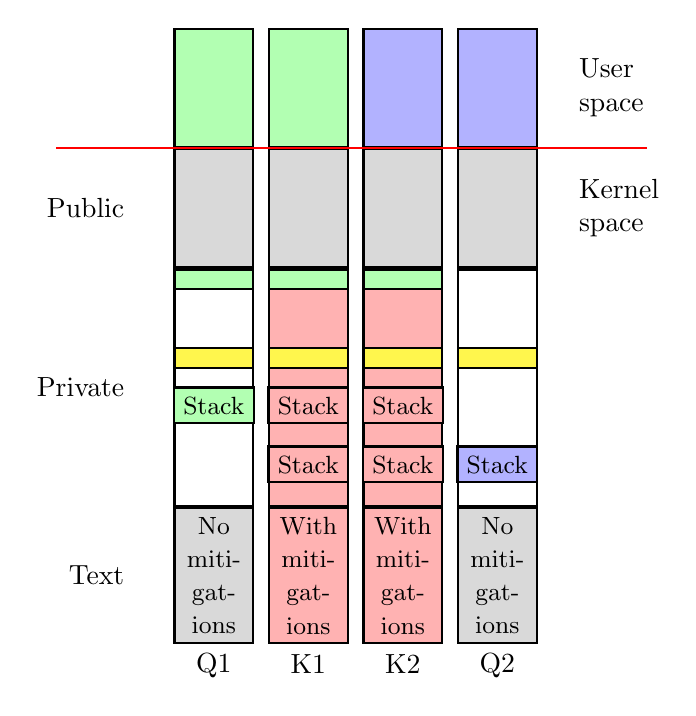
\begin{tikzpicture}[>=latex]

  \tikzstyle{A}=[thick,rectangle, draw, minimum width=1cm,minimum
    height=1.5cm, align=center];
  \tikzstyle{Q1}=[thick,rectangle, draw, minimum width=1cm,minimum
    height=1.5cm, align=center,fill=green!30];
  \tikzstyle{Q2}=[thick,rectangle, draw, minimum width=1cm,minimum
    height=1.5cm, align=center,fill=blue!30];
  \tikzstyle{K}=[thick,rectangle, draw, minimum width=1cm,minimum
    height=1.5cm, align=center,fill=red!30];
  \tikzstyle{BIG}=[minimum height=3cm];
  
  \node [Q1,fill=gray!30] (q1) {};
  \node [Q1,xshift=1.2cm,fill=gray!30] (qk1) {};
  \node [Q2,xshift=2.4cm,fill=gray!30] (qk2) {};
  \node [Q2,xshift=3.6cm,fill=gray!30] (q2) {};
%  \node [K,xshift=4.8cm,fill=gray!30] (k) {};

  \node [left=of q1.west,align=left,xshift=.5cm] (u) {Public};

  \node [Q1,BIG,below=of q1.south,yshift=1cm,fill=white] (q11) {};
  \node [K,BIG,below=of qk1.south,yshift=1cm] (qk11) {};
  \node [Q2,BIG,below=of q2.south,yshift=1cm,fill=white] (q21) {};
  \node [K,BIG,below=of qk2.south,yshift=1cm] (qk21) {};
  
  \node [Q1,below=of q1.south,yshift=1cm,minimum height=0.25cm] (q11a) {};
  \node [K,below=of qk1.south,yshift=1cm,minimum height=0.25cm,fill=green!30] (qk1a) {};
  \node [K,below=of qk2.south,yshift=1cm,minimum height=0.25cm,fill=green!30] (qk2a) {};

  \node [Q1,below=of q1.south,yshift=0cm,minimum height=0.25cm,fill=yellow!70] (q21b) {};
  \node [K,below=of qk1.south,yshift=0cm,minimum height=0.25cm,fill=yellow!70] (qk1c) {};
  \node [K,below=of qk2.south,yshift=0cm,minimum height=0.25cm,fill=yellow!70] (qk2c) {};
  \node [Q2,below=of q2.south,yshift=0cm,minimum height=0.25cm,fill=yellow!70] (q21b) {};

  \node [Q1,below=of q1.south,yshift=-0.5cm,minimum height=0.25cm] (q11s1) {\small Stack};
  \node [K,below=of qk1.south,yshift=-0.5cm,minimum height=0.25cm] (qk1s1) {\small Stack};
  \node [K,below=of qk2.south,yshift=-0.5cm,minimum height=0.25cm] (qk2s1) {\small Stack};

  \node [K,below=of qk1.south,yshift=-1.25cm,minimum height=0.25cm] (qk2s2) {\small Stack};
  \node [K,below=of qk2.south,yshift=-1.25cm,minimum height=0.25cm] (qk2s2) {\small Stack};
  \node [Q2,below=of q2.south,yshift=-1.25cm,minimum height=0.25cm] (q21s2) {\small Stack};
  
%  \node [K,below=of k.south,yshift=1cm,minimum height=0.25cm,fill=green!30] (k1a) {};
%  \node [K,below=of k1a.south,yshift=1cm,minimum height=1.0cm] (k1b) {};
%  \node [K,below=of k1b.south,yshift=1cm,minimum height=0.25cm,fill=blue!30] (k1c) {};

  \node [left=of q11.west,align=left,xshift=.5cm] (u) {Private};

%  \node [Q1,below=of q11b.south,yshift=0cm] (q12) {};
%  \node [K,below=of qk1c.south,yshift=0cm] (qk12) {};
%  \node [Q2,below=of q21b.south,yshift=0cm] (q22) {};
%  \node [K,below=of qk2c.south,yshift=0cm] (qk22) {};
  
%  \node [K,below=of k1c.south,yshift=1cm] (k2) {};

%  \node [left=of q12.west,align=left] (u) {Stack};
  
  \node [Q1,below=of q11.south,yshift=1cm,fill=gray!30] (q13) {\small No \\ \small miti- \\ \small gat- \\ \small ions};
  \node [K,below=of qk11.south,yshift=1cm] (qk13) {\small With \\ \small miti- \\ \small gat- \\ \small ions};
  
  \node [Q2,below=of q21.south,yshift=1cm,fill=gray!30] (q23) {\small No \\ \small miti- \\ \small gat- \\ \small ions};
  \node [K,below=of qk21.south,yshift=1cm] (qk23) {\small With \\ \small miti- \\ \small gat- \\ \small ions};
  
%  \node [K,below=of k2.south,yshift=1cm] (k3) {};

  \node [left=of q13.west,align=left,xshift=.5cm] (u) {Text};

  %% user space
  
  \node [A,above=of q1.north,yshift=-1cm,fill=green!30] (a1) {};
  \node [A,above=of q2.north,yshift=-1cm,fill=blue!30] (a2) {};

  \node [A,above=of qk1.north,yshift=-1cm,fill=green!30] (a11) {};
  \node [A,above=of qk2.north,yshift=-1cm,fill=blue!30] (a21) {};

  \draw[thick,color=red] (q1.north) ++(-2cm,0) -- ++(7.5cm,0)  node {};

  \node [right=of a1.east,xshift=3cm,align=left] (u) {User\\space};
  \node [right=of q1.east,xshift=3cm,align=left] (k) {Kernel\\space};

  \node [below=of q13.south,yshift=1cm,align=left] {Q1};
  \node [below=of qk13.south,yshift=1cm,align=left] {K1};
  
  \node [below=of q23.south,yshift=1cm,align=left] {Q2};
  \node [below=of qk23.south,yshift=1cm,align=left] {K2};
  
%  \node [below=of k3.south,yshift=1cm,align=left] {K};
  
\end{tikzpicture}


  \end{center}
  \vspace{-2\baselineskip}
  \caption{Overview of \sys's address space layout with two processes
    (indicated by the colors green and purple). Each process has a Q
    and K domain. Q domains have access to public data (the grey
    color) and per-process kernel data; the
    white private region is unmapped kernel data. Each domain also has
    its own stack and kernel text. In the Q domain, the kernel text
    has no mitigations. The K domains map all memory, including
    sensitive memory (indicated by red); all K domains have the same
    memory layout. Data structures that are shared across processes,
    such as pipes or file pages, can be mapped in multiple Q domains,
    as indicated by the yellow color.}
\label{fig:overview}
\end{figure}

\sys's design maintains two page tables per process.  One page table
defines a process-specific view of kernel memory.  When a process is
running with that page table, we say it is running in its
\textit{quasi-visible} domain (or Q domain for short), and with its Q page
table.  Following the unmapped speculation contract, \sys assumes any
kernel memory mapped by the Q page table can be leaked to the
currently running process.  Instead of using mitigations to prevent
leaks of kernel memory, \sys arranges for the mappings in the Q page
table to be such that they contain no sensitive data of other
processes.

When the process needs to access data that is not mapped in the Q page
table, it can switch to its other page table, which maps all physical
memory, including memory that contains sensitive data.  When a process
is running with this page table, we say the process is executing in
its \textit{K} domain with its K page table.  In its K domain, the process
runs with the same mitigations as Linux currently uses.

This design allows many system calls to execute in the Q domain,
with no mitigation overhead.  As a simple example,
\texttt{getpid} does not access any sensitive data; it needs
access to only the kernel text and its own process structure.  A more
interesting example is mapping anonymous memory: it requires access
to the process's own page table and to the memory allocator, but not
other processes' page tables or pages.

\autoref{fig:overview} shows the address space layout in \sys in more
detail.  Each process has a Q and K view of memory.  When a process is
running in user space it runs in its Q domain (with no secrets mapped
in the Q page table).  When a user process makes a system call it
enters the kernel but stays in its Q domain.  The Q domain maps public
kernel memory, Q-visible kernel memory, the process's Q domain stack,
and the kernel text without mitigations.

If a system call needs access to memory in the K domain, \sys performs a
switch from its Q domain to its K domain. We refer to the switch from a Q
domain to a K domain as a \textit{world switch}, because kernel code in
a Q domain runs without most mitigations and the kernel code in the K domain
runs with full mitigations. Furthermore, the process switches from its
Q domain stack to its K domain stack.  The K domain, with access to
all kernel memory, can then execute the rest of the system call with
full mitigations.

Achieving good performance in \sys depends on avoiding world switches.
To reduce the number of world switches, \sys maps kernel data
structures that contain no sensitive data into every Q domain.  For
example, all Q domains map x86 configuration tables (IDT, GDT), some
memory allocator state, etc.  On the other hand, kernel data structures
that contain application data, such as process memory or saved register
state, are not mapped into Q domains unless that process should have
access to that data.

\subsection{World switch}
\label{ss:switch}

One of the challenges in \sys's design is that a system call often does
not know upfront whether it will need to execute in the Q domain or in
the K domain.  For example, a \texttt{read} system call might be able to
execute purely in the Q domain, or might need access to sensitive data
from the K domain, depending on the file descriptor that the process is
reading from, and depending on whether this Q domain already has some
sensitive data mapped or not.  To support this, \sys's design allows
a system call to start executing in the Q domain, and switch to the K
domain later as needed.

\sys allows the Q domain to trigger a world switch either
\textit{intentionally} or \textit{transparently}.  If the code
determines that it must switch to the K domain, it can intentionally
invoke the function, \texttt{kswitch()}, to perform a world switch.
When \texttt{kswitch()} returns, the kernel thread is now executing in
the K domain, and has access to all memory.  If the Q domain needs
access to specific sensitive data which might or might not be already
mapped, the Q domain can attempt to access the virtual address of that
data.  If the data is already mapped in the Q domain, the access will
succeed, no world switch happens, and the Q domain can continue
executing.  If the data is not mapped, the Q domain triggers a page
fault, which transparently triggers a world switch.  Once the page
fault returns, the kernel thread is now executing in the K domain, as
if it called \texttt{kswitch()}.  Compared to making an intentional
call to \texttt{kswitch()}, the transparent approach incurs a slight
overhead for executing the page fault, but allows large sections of
the kernel to be kept completely unmodified, and allows the Q domain
to elide a world switch altogether if the data is already mapped in
the Q domain.

The above design requires that a kernel thread can start executing in
the Q domain and transparently switch to executing in the K domain.
This means that any addresses that the kernel thread is referencing,
including pointers to data structures, stack addresses, and function
pointers, remain the same.  To achieve this, \sys ensures that the
layout of the Q domain and the K domain match.  In particular, all
data structures in the Q domain must appear at the same address in the
K domain, and the kernel code (text) is located at the same address
(even though the code is slightly different, as described in \autoref{ss:ktext}).

The stack requires particular care because a kernel thread that is
processing sensitive data in the K domain could inadvertently write
that data to the stack.  For example, a \texttt{read()} system call
from \texttt{/dev/random} needs to switch to the K domain to access the
system-wide randomness pool.  However, the pseudo-random generator code
might spill some of its state to the stack, depending on the compiler's
choices.  If the stack is accessible from the Q domain, the sensitive
data could in turn be leaked during the next entry into the Q domain by any
thread within the same process.  At the same time, if the
K domain stack was separate from the Q domain stack, pointers to stack
locations before a world switch would no longer work after a world switch.
To reconcile these constraints without having to rely on any dedicated
compiler support, \sys maps a distinct kernel stack for each domain at the
virtual address range and copies the Q domain stack contents to the K domain
stack during a world switch.


\subsection{Mitigations}
\label{ss:mitigations}

% \fk{this section needs to be fleshed out and needs careful review}

\begin{figure}
\centering
\small
\begin{tabular}{lccc}
{\bf Transient execution vulnerability} & {\bf User/Q-domain} & {\bf K-domain} & {\bf Context Switch} \\

\midrule
L1TF & x & x & \\

\midrule
V1 (Bound Check Bypass) & & x & \\
V1.1 (Bounds Check Bypass Store) & & x &\\
V3 (Meltdown) && x &\\
V4 (Speculative Store Bypass) &	 & x &  \\

\midrule
V2 (Branch Target Injection) & & x & x \\
Microarchitectural Data Sampling && x & x\\
\qquad (Fallout, RIDL, Zombie Load, etc.) \\

\midrule

LazyFPU &&& x \\
SpectreRSB &&& x\\

\midrule
PortSmash & \multicolumn{3}{c}{Not applicable} \\
Load Value Injection & \multicolumn{3}{c}{Not applicable} \\
Meltdown-PK (protection key bypass) & \multicolumn{3}{c}{Not applicable} \\
Meltdown-BR (bounds check instr. bypass) & \multicolumn{3}{c}{Not applicable} \\
V1.2 (Read-only Protection Bypass) & \multicolumn{3}{c}{Not applicable} \\

\end{tabular}
\caption{The mitigations implemented in software by \sys{}.}
\label{fig:mitigations}
\end{figure}

\autoref{fig:mitigations} shows the known transient execution
attacks~\cite{hill:survey,sok:transient}, organized by the mitigations
needed to address those attacks in \sys's design.  The columns indicate where the mitigations are needed: while
executing in user-mode or the Q domain; while executing in the K domain;
and when context-switching between processes.

% The first attack, System Register Read, requires mitigation in user-space
% to prevent adversarial processes from obtaining the contents of sensitive
% system registers.  However, no mitigation is required when running in
% the K domain, since we do not expect the K domain to issue speculative
% system register reads (much as in Linux).

The L1TF attack allows leaking the contents of the L1 cache if
there are partially-filled-in entries in the page table.  We think of
this attack as a violation of the USC (see \autoref{fig:attack-by-state}),
but a simple microcode fix, as well as clearing unused page table entries,
makes the system agree with the USC, and avoids the L1TF attack.  Since
L1TF allows leaking the contents of any data, \sys applies the mitigations
both in user-space, Q domain, and K domain.

The next category of attacks requires no mitigations in either user-space
or Q domain.  Specifically, Spectre variants that bypass bounds checks
require mitigation in the K domain, since there is sensitive memory
contents that could be leaked as a result of a speculative check bypass.
However, there is no sensitive data that can be leaked in the Q domain,
owing to \contract{}.  Similarly, no mitigations are required on a
context switch, since these attacks can only leak data from the current
protection domain.

Meltdown also falls in this category, but for a different reason.
Meltdown allows an adversary to bypass the user-kernel boundary check
in the page table.  \sys's use of a separate page table for the Q and
K domains ensures that Meltdown cannot leak any confidential data, since
no confidential data is available in the Q domain.  Recent fixes from Intel resolve the Meltdown attack in a way that avoids the need for
software mitigations.

The next category of attacks require mitigation both in the K domain and
on context switch.  Spectre v2 and MDS attacks can allow an adversary to
obtain sensitive data either from the OS kernel or from another process.
However, no mitigations for these attacks are needed in the Q domain
due to \contract{}: there is no sensitive data to leak in the Q domain
of the currently running process.

For some attacks, such as LazyFPU and SpectreRSB, mitigations are only
required on context switch, because the attacks involve process-to-process
leakage.

Finally, a number of attacks are not applicable to \sys's simpler design,
in contrast to Linux.  For example, \sys does not support SGX, does
not support running virtual machines, and does not use certain hardware
features (such as hardware bounds-check instructions or protection keys).


\subsection{Kernel text}
\label{ss:ktext}

Some of the mitigations involve changes to the executable kernel code
(text), such as the use of retpolines in place of indirect jumps.
These mitigations impose a performance cost, but they are not needed
when executing in the Q domain.

A na\"ive approach might be to compile the kernel code twice, with
different compiler flags for mitigations, and load the two different kernel
binaries in the Q and K domains respectively. However, this would break \sys's
page fault triggered world switches because after completing the switch,
execution would resume with the same instruction pointer and stack contents
from before the switch but neither would be meaningful in the new text
segment.

Instead we need the two version to have matching instruction addresses and stack
layouts. \sys achieves this by compiling the kernel only once, but then making
two copies of the code at runtime. One copy is mapped into all the K domains,
and the other into all the Q domains \textit{but at the same virtual address
as in the K domains}. Switching between the two is seamless.

At boot time, in a process inspired by Linux's \textsc{alternative}
macro~\cite{lwn:alternative}, \sys locates each \texttt{call} or
\texttt{jmp} in the Q text segment pointing to a retpoline thunk, and
replaces them with the instruction that retpoline emulates. One
complication is that indirect call instructions are only 2 or 3 bytes,
compared to the 5 that a direct call instruction takes. If we tried
to pad with a \texttt{NOP} instruction before or after, the pair would not execute
atomically, so instead we prepend indirect calls with several
repetitions of the CS-segment-override prefix, which is always ignored
in 64-bit mode.


\subsection{Memory management}
\label{ss:mm}

Memory allocation in \sys is complicated by the fact that the contents
of free pages may contain sensitive data.  In particular, if a page was
freed by one process, its contents must be erased before the page can
be mapped in another Q domain.  Zeroing out pages on every allocation
would be costly, in particular when allocating kernel data structures,
which do not otherwise require the memory to be zero-filled.

To avoid the overhead of repeatedly zeroing kernel pages, \sys implements
a sharded allocator for kernel memory.  Each Q domain has its own pool
of pages for allocation, and the K domain keeps all of the kernel memory
that is not part of any Q domain.  \sys transfers memory between these
shards in batches to amortize the world switch overhead.  Keeping a pool
of kernel memory in a Q domain allows the kernel to repeatedly allocate
and free memory within a Q domain with little overhead.

The other category of memory managed specially by \sys is public memory.
\sys maintains a single pool of public pages, with separate functions,
\texttt{palloc()} and \texttt{pfree()}, for allocating and freeing in
that pool.  All public-pool pages are mapped in every Q domain.


\subsection{Process management}
\label{ss:proc}

When the \sys kernel switches from executing one process to another, it
must perform a world switch, to ensure that confidential data does not
leak across processes (such as the saved CPU registers that the kernel
might save on the stack).  However, if a multi-threaded application
is running, there is no security reason to perform a world switch when
switching between multiple threads in the same process---all of the
threads have the same privileges and have access to the same process
address space.

To avoid mitigation overhead when switching between threads in the
same process, \sys splits the process descriptor, \texttt{struct
  proc}, into two parts.  The first part stores sensitive process
state, such as the saved CPU registers, and is not public.  The second
part stores metadata about the process, such as the PID, the run
queue, the scheduler state, etc.  This part is public and is used by
the scheduler when deciding what thread to execute next.  As a result,
the scheduler can pick the next thread without incurring a world
switch.  Furthermore, if the next thread happens to be from the same
process, the context switch code can also avoid performing a world
switch.  Existing scheduler policies that favor picking threads from
the same process mesh well with this approach.

\subsection{File system}
\label{ss:fs}

File system workloads involve access to several kernel data structures,
including the inode cache and the page cache (containing file data).
Inodes are challenging for \sys to deal with because they are smaller than
a page, so it is not feasible to map them individually into a Q domain.
However, achieving good performance for file system operations requires
being able to access an inode without a world switch.  To reconcile
this conflict, we chose to make all inode structures public in \sys,
similar to our approach for splitting the \texttt{proc} structure above.
If the inode had sensitive data (such as extended attributes), that
part of the inode structure would need to be split off into a separate
private structure, along the lines of how we split off the part of the
\texttt{proc} structure storing saved CPU registers.

File data pages are not public, because their contents might be sensitive.
\sys implements an optimization that allows it to access file
contents without a world switch.  In particular, after \sys checks
the permissions on a file, it reads or writes the contents of a file
page by temporarily mapping the corresponding physical page of memory
into its Q domain's address space.  This allows the Q domain to access
that specific memory page without the risk of leaking other pages;
as a result, no mitigations or world switches are needed.  When the Q
domain is finished with the file read or write, it unmaps the page and
issues a TLB shootdown, in case the file is later truncated and the page
gets reused for other data.


\subsection{Pipes}

Pipes are different from many of the other kernel data structures discussed so
far in that their contents shouldn't be visible globally, but their state can be
associated with multiple processes at a time. \sys's goal is to ensure that if a
reader and writer of a pipe run on different cores, then they don't incur world
switches when they access the pipe. To achieve this, we store a pipe's data
structures in shared memory regions between Q domains. These shared regions are
lazily mapped into Q domains the first time a process accesses a pipe (doing the
mapping on \texttt{fork} would cause unnecessary overhead), and unmapped when
the last reference to the pipe within a Q domain is closed. 

When a pipe becomes full or empty, the caller blocks on a condition
variable. Subsequent reads or writes can observe which processes are blocked and
add them to the scheduler run queue if appropriate. Neither of these operations
requires access to any secret data so no world switch is triggered until a new
process is scheduled. Thus, if the core remains idle until the blocking thread
is added back to the run queue, the cost of a world switch is avoided.

\subsection{Discussion}

\sys's design assumes that there are no secrets in the Q domain that
need to be hidden from the user-level process.  For many secrets, they
can be protected by placing them in the K domain, such as the seed
of a system-wide randomness generator.  However, address-space layout
randomization (ASLR) for the kernel address space is difficult to protect
in this fashion, because kernel addresses must be used in the Q domain,
and the addresses must match up between the Q domain and the K domain
in order for world switches to work.  (Note that the initial seed that
is used to randomize layout could be protected in the K domain, but the
resulting randomized layout cannot be protected.)  As a result, kernel
ASLR in \sys is susceptible to leakage of addresses through transient
execution side-channels.

Our \sys prototype does not include an optimized in-kernel network stack, but a
reasonable approach might be to treat all network data as public, leaving
it up to the application to encrypt any sensitive information sent over
the network.  This meshes well with the recent trends in widespread use
of TLS for network security, and allows for network operations to achieve
high performance in \sys because no mitigations or world switches are
required, and all network processing can stay in the Q domain.

Hyperthreading is a source of many possible transient execution leaks,
because a significant amount of microarchitectural state is shared
between the execution contexts.  However, many Linux systems continue
to run with hyperthreading \emph{enabled}, despite these risks, because
of the high performance overhead they would incur if hyperthreading was
entirely disabled.  \sys does the same.

\section{Implementation}
\label{s:impl}

\begin{figure*}
\centering
\small
\begin{tabular}{lll}
{\bf Transient execution variant} & {\bf Strategy} & {\bf Support} \\
\midrule
V1 (Bound Check Bypass) & bounds clipping & partial \\
V1.1 (Bounds Check Bypass Store) & lfence & partial \\
V1.2 (Read-only Protection Bypass) & lfence & n/a (no in-kernel software sandbox) \\
V2 (Branch Target Injection) &	retpoline & yes \\
\quad \ditto & speculation barrier	&	yes \\
\quad \ditto & return stack buffer filling	&	yes \\
\quad \ditto & disable spec before BIOS calls &	n/a (no calls to BIOS in \sys) \\
V3 (Meltdown) & Kernel page table isolation (KPTI) &	yes \\
V3a (System Register Read) & microcode & yes \\
V4 (Speculative Store Bypass) &	disable spec. or ctx. switch & yes \\
LazyFPU	& hardware-assisted save/restore & yes \\
SpectreRSB & return stack buffer filling & yes \\
L1TF &	cache flush, no SMT & 	n/a (no VM entry in \sys)  \\
\quad \ditto & no invalid PTEs	&	yes \\
PortSmash & no SMT  &	no \\
Microarchitectural Data Sampling  & CPU buffer clearing & yes \\
(Fallout, RIDL, Zombie Load, etc.) & no SMT &	no \\
Load Value Injection & lfence &	n/a  (no SGX in \sys) \\
Meltdown-PK 
(protection key bypass)
& address space isolation & n/a (no protection keys) \\
Meltdown-BR
(bounds check instr. bypass)
& lfence & n/a (no bounds check instructions) \\
\end{tabular}
\caption{Transient execution mitigations implemented in \sys.}
\label{fig:mitigations-impl}
\end{figure*}

To demonstrate the feasibility of the \sys design, we implemented a
prototype of \sys starting from the sv6 research kernel. The kernel
  is monolithic, implementing traditional OS services such as virtual
  memory, processes and threads, file systems, fine-grained
  concurrency using RCU-like techniques, etc.  The sv6 kernel, is
  written in C/C++, runs on x86 processors (both AMD and Intel), and
  has decent uniprocessor performance and great multicore performance
  and scalability~\cite{clements:sc}.

\paragraph{Kernel changes.}

\sys's design affects most core kernel subsystems, including the memory
allocator, virtual memory, context switching and the scheduler, and the
file system.  The simplicity of sv6 allowed for rapid experimentation
with kernel designs to enable \sys, which would have been challenging
to do in a more complex kernel like Linux, since it is time-consuming
to make changes to core subsystems in the Linux kernel, which would have made
design iterations far slower.

To help partition the kernel data structures across Q domains, we
developed Warden, a tool for tracking down the cause of world switches.
Warden instruments page faults from the Q domain that lead to a
world switch, and records a stack trace for each of them.  Examining the
profile of these world switches allows the kernel developer to quickly
understand what kernel data structures need to be partitioned or sharded
to reduce the number of world switches, as well as the operations
that need to be supported on these data structures within a Q domain.
Although Warden identifies the data structures that are causing world
switches, it is up to the kernel developer to identify an appropriate
plan for partitioning the data structure so that no sensitive data can
leak through side channels.

To run applications on top of the \sys prototype kernel, we changed the
\sys system call interface, including system call numbers, data structure
layout, etc, to match that of Linux.  This allows unmodified Linux
ELF executables to run on top of \sys, and ensures that \sys implements
(a subset of) the same system calls that are available on Linux.

We modified sv6 to use PCIDs to reduce the cost of switching page
tables (see \autoref{ss:switch}).  To improve TLB shootdown
performance, we modified sv6 to use Linux's shootdown strategy.  This
is important, for example, for removing temporary mappings in a
\texttt{read} and \texttt{write} systems calls (see \autoref{ss:fs}).

\paragraph{Mitigations.}

\sys implements side-channel mitigations for known transient
execution attacks~\cite{hill:survey,sok:transient}, as shown
in \autoref{fig:mitigations-impl}.  \sys mostly copies the
mitigation strategies and their implementation from the Linux
kernel~\cite{linux:vuln}; the most interesting exception is that \sys
does not apply some of these mitigations to the Q domain, as described
in \autoref{fig:mitigations}.

For Spectre V1, \sys, adds an \texttt{lfence} instruction when copying
from user code, and when taking an interrupt, exception, and NMI entry.
\sys uses bounds clipping in fewer cases than Linux for two reasons:
\sys has less code and we haven't performed a careful audit of the
complete source code.  For Spectre V2, we compile \sys to use retpolines
(by specifying the ``-mretpoline-external-thunk'' flag to \texttt{clang}). \sys
also uses Linux's \texttt{FILL\_RETURN\_BUFFER} macro to fill the
return stack buffer, and issues an indirect branch predictor barrier
\texttt{IBPB} instruction on a context switch. For Spectre V3, \sys uses
separate page tables (as described in \autoref{ss:overview}) and uses
process-context identifiers (\texttt{PCID}s) to avoid TLB flushes.

For Spectre V4, \sys issues an \texttt{lfence} on context switch. (If
\sys supported generating code at runtime, the JITs would also have to
be hardened.)  For LazyFPU, \sys uses the \texttt{xsaveopt}
instruction to safe/restore floating point state.  For SpectreRSB,
\sys fills the return stack buffer on context switch.  For L1TF, \sys
avoids invalid PTEs. Like Linux, \sys doesn't address PortSmash; the
default for the Linux kernel is to allow SMT, and \sys does too.  For
microarchitectural data sampling attacks, \sys issues the
\texttt{verw} instruction for clearing CPU buffers.

Some attacks aren't applicable to \sys, because \sys doesn't support
virtualization, secure enclaves, and hardware transactional memory;
does not call into the BIOS; and does not implement in-kernel software
sandboxes such as BPF.

Like Linux, \sys also zeroes unused CPU registers on kernel entry, to
reduce the avenues of attack available to an adversary.  To determine
whether mitigations are necessary, \sys maintains a special variable
called \texttt{secrets\_mapped} whose value is 0 in the Q domain and 1 in
the K domain; this allows the rest of the kernel code to determine if it
needs to perform mitigations just by using \texttt{if (secrets\_mapped)
...} (as long as interrupts are disabled, to avoid races).  To help
evaluate the performance impact of side-channel mitigations, \sys's
implementation allows switching individual mitigations on and off at
runtime, rather than at compile time or boot time.

To improve performance, a few system calls invoke the world switch
intentionally to avoid the extra overhead of a transparent world switch.
For example, \texttt{open}, and \texttt{fork} always
invoke world switch intentionally.  The \texttt{read} and \texttt{write}
system calls invoke a world switch intentionally when they are reading
or writing large amounts of data, since the cost of a world switch is
less than the cost of shooting down the temporary mappings for that many
file pages.  A page fault on a Copy-On-Write (COW) page also intentionally
invokes a world switch.


\paragraph{Lines of code.}

The \sys prototype consists of about 34,000 lines of C++ code (for
\texttt{kernel/} and \texttt{include/}), compared to 24,000 lines of
C++ code for the sv6 kernel that \sys was derived from.
\texttt{git diff --stat} reports roughly 17,000 lines of insertions and 5,000
lines of deletions between sv6 and \sys.
It is difficult to further
break down \sys's lines of code, since many aspects of \sys's design
required small changes throughout the kernel's source code.  For
example, splitting up the kernel memory allocator required the use of
C++ placement \texttt{new} in many parts of the kernel.  Similarly,
implementing the Linux binary compatibility layer required making
changes to the implementation of many system calls.


\section{Evaluation}
\label{s:eval}

To demonstrate the benefits of \sys's design, this section
answers the following questions:

\begin{itemize}

\item Do \sys's techniques reduce the overhead of mitigations for
system calls?  (\autoref{ss:faster})

\item How do mitigations affect the cost of a world switch?
  (\autoref{ss:world})

\item What are the memory overhead associated with \sys's design?
  (\autoref{ss:memoverhead})

%\item Does \sys's use of the unmapped speculation contract address
%  known transient execution vulnerabilities?  (\autoref{ss:secure})

%% \item Could \sys's design reduce overhead for Linux's systems calls?
%%   (\autoref{ss:linux})
 
\end{itemize}

\begin{figure*}[ht]
  \begin{center}
    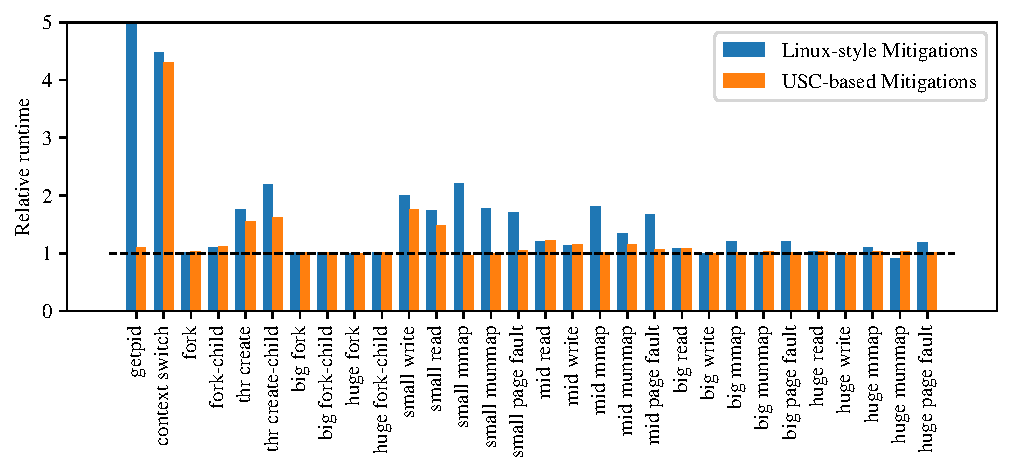
\includegraphics{results/ward_overhead_lebench}
  \end{center}
\vspace{-\baselineskip}
\caption{Performance of \sys with fast USC-based mitigations and with Linux-style mitigations,
  normalized against the baseline performance of \sys without any mitigations.}
\label{fig:slowdown}
\end{figure*}


\subsection{Experimental methodology}

To answer these questions, we consider three different configurations of \sys:

\begin{itemize}
\item Baseline: \sys with no mitigations against side channels.

\item Linux-style: \sys with standard mitigations against side channels,
mirroring the approach taken by the Linux kernel.  This configuration does
not use separate Q domains; all system calls directly enter the K domain.

\item USC-based: \sys with fast mitigations that take advantage of the split
between the Q domain and the K domain, leveraging the \contract{}.  The
K domain implements the same mitigations as in Linux-style.

\end{itemize}

\sys's design is aimed at reducing the overhead of mitigations
associated with system calls.  To zoom in on the system call overhead,
we evaluate \sys's performance using \bench~\cite{lebench}, a
collection of system call workloads representative of a range of real
applications.  This allows us to precisely report and explain the
effect of \sys's techniques on individual system calls.  We don't
report results for the networking benchmarks in \bench, because the
\sys prototype doesn't have a suitable in-kernel network stack.

All benchmarks were run on a Dell PowerEdge T430 with two E5-2640 v4
CPUs and 64 GB of RAM.

%% All benchmarks were run on a 4th Gen Lenovo X1 Carbon Laptop with a Intel
%% i7-6600U CPU and 16 GB of RAM. Except where otherwise noted, we ran with the
%% latest available microcode for our processor (released on Nov 15, 2019).
%% \nz{XXX update to describe bhw2 hardware.}

One potential concern with the use of recent microcode is that it makes
the baseline slower, which in turn makes the cost of mitigations appear
lower than they really are.  This is similar to the significant effect
we observed with newer CPUs, as described in \autoref{s:motivation}.
However, with newer microcode, we find that the performance of the
baseline is not significantly affected: it achieves similar performance
even when we use old microcode.  The reason for this is that the recent
microcode updates add mitigations that can be specifically enabled (e.g.,
through the \texttt{SPEC\_CTRL} MSR), but almost nothing is enabled by
default.  The Linux and Ward baseline experiments do not enable these
mitigations, and thus the performance effect is minimal.
%\nz{perhaps verify this also on bhw2, since we did this experiment
%originally on jonathan's laptop}

For the Linux measurements of \bench, we use the 5.4.0 kernel on Ubuntu 20.04.


\subsection{\sys's USC-based fast mitigations}
\label{ss:faster}

\paragraph{\bench.}

\autoref{fig:slowdown} shows the benefit of \sys's fast mitigations on
\bench.  The figure compares \sys with USC-based and Linux-style mitigations,
relative to the baseline with no mitigations.
As shown, \sys with fast USC-based mitigations is often able to
match the unmitigated baseline.  The reason is that many of the microbenchmarks can
execute with no or very few world switches, as shown in
\autoref{fig:count}.

Many microbenchmarks (\texttt{getpid} through \texttt{huge pagefault}
in \autoref{fig:count}) have nearly 0 transparent and intentional
world switches. They execute completely in the Q domain. The
reason that some have near 0 world switches, but not exactly 0, is
that during the measurement they were interrupted by a timer
interrupt, which requires a world switch to the K domain to run the
scheduler (the remainder of the syscall is then executed in the K
domain too).

Another cause for fractional numbers of transparent world
barriers is that some operations might have a slow path that requires
secrets but only gets triggered infrequently (i.e. because a memory
allocator pool ran empty). A strength of the \sys approach is that these
sorts of cases don't have to be manually annotated and in fact it is
harmless to completely ignore them provided they are executed infrequently
enough.

There are several microbenchmarks (e.g., the bigger \texttt{read} and
\texttt{write} ones) that perform one intentional world switch per
system call.  These system calls immediately enter the K domain and
thus perform identical to \sys with full mitigations, and have the
same overhead.  These system calls also perform much work in the kernel and
the overhead of the 1 world switch is amortized by that work.

\begin{figure}
\small
\centering
\begin{tabular}{lrccc}
  & {\bf \# sys calls} & \multicolumn{3}{c}{{\bf World switches}} \\
  & & {\bf T} & {\bf I} & {\bf Sum}  \\
  \midrule
getpid & 1 & 0 & 0 & 0 \\
small write & 1 & 0 & 0 & 0 \\
small read & 1 & 0 & 0 & 0 \\
small mmap & 1 & 0 & 0 & 0 \\
small munmap & 1 & 0 & 0 & 0 \\
small page fault & 1 & 0 & 0 & 0 \\
mid mmap & 1 & 0 & 0 & 0 \\
mid munmap & 1 & 0 & 0 & 0 \\
mid page fault & 1 & 0 & 0 & 0 \\
big mmap & 1 & 0 & 0 & 0 \\
big page fault & 1 & 0 & 0 & 0 \\
huge mmap & 1 & 0 & 0 & 0 \\
huge page fault & 1 & 0 & 0 & 0 \\
context switch & 2 & 0 & 1 & 1 \\
thr create & 3 & 0 & 1 & 1 \\
thr create-child & 4 & 0 & 1 & 1 \\
mid read & 1 & 0 & 1 & 1 \\
mid write & 1 & 0 & 1 & 1 \\
big read & 1 & 0 & 1 & 1 \\
big write & 1 & 0 & 1 & 1 \\
big munmap & 1 & 1 & 0 & 1 \\
huge read & 1 & 0 & 1 & 1 \\
huge write & 1 & 0 & 1 & 1 \\
huge munmap & 1 & 1.001 & 0 & 1.001 \\
fork & 2 & 0 & 2 & 2 \\
big fork & 2 & 0 & 2 & 2 \\
huge fork & 2 & 0 & 2 & 2 \\
huge fork-child & 17 & 0 & 7 & 7 \\
big fork-child & 17 & 0.006 & 7.02 & 7.026 \\
fork-child & 17 & 0.012 & 7.065 & 7.077 \\
\end{tabular}
\caption{The microbenchmarks, sorted by the sum of the number of transparent
  ({\bf T}) and intentional ({\bf I}) world switches per iteration, along
  with the number of system calls invoked (including page faults).}
\label{fig:count}
\end{figure}

The \texttt{thr create} and \texttt{thr create-child} do multiple syscalls
per iteration, but average  one world barrier per iteration.
Specifically, the \texttt{thr create} microbenchmark makes three systems calls:
one \texttt{clone} that requires a world switch and a call to each of
\texttt{sigprocmask} and \texttt{set\_robust\_list} which don't. The
\texttt{thr create-child} microbenchmark includes an additional call to
(\texttt{sigprocmask}) from the child process, for which \sys can also
avoid the world switch.

The \texttt{fork} and \texttt{fork-child} benchmarks each do a single syscall
with an intentional world barrier that takes the vast majority of execution time,
but also raise a handful of page faults to populate page table entries (which
need secrets if they are copy-on-write related or if the kernel runs out of
zeroed memory pages and has to prepare more).

An interesting case is the \texttt{context switch} microbenchmark.
This microbenchmark measures context switching by writing and reading
a byte over a pipe between two processed pinned to the \textit{same}
core. The \texttt{write} calls avoids a world switch because the
scheduler can wake other processes while in the Q domain, but the
\texttt{read} call causes a context switch and (since the two
processes are mutually distrusting) thus requires a world switch.

When we modify the microbenchmark to pin the two processes to \textit{different}
cores we observe that it runs without world switches and that the overhead is about 25 times lower than Linux-style mitigations.

%% When measuring context switching overhead for ping-ponging a futex between two
%% threads of a user-level process, fast mitigations improve performance: fast
%% relative to no mitigations has a performance slow down of 1.14$\times$, while
%% standard mitigations have a slow down of 2.79$\times$. \jb{Replace with pipes
%%   benchmark}

%% schedbench.csv


\paragraph{Application: git.}

To confirm that the improved performance of \sys's fast mitigations seen
in \bench translates into application-level performance improvements,
we evaluated the performance of \texttt{git}.  For this benchmark, we
ran \texttt{git status} in a 100 MB repository that we cloned from
GitHub; all of the file system
state was cached in memory. The average runtime for Linux-style mitigations
took 24.6\%
longer than the unmitigated baseline, and USC-style mitigations took 11.2\% longer than
the unmitigated baseline.
Much of the speedup is due to the fact that \texttt{git status} invokes
frequent \texttt{lstat} system calls, which can execute in the Q domain.
The remaining overhead is due to system calls like \texttt{openat} that
require a world barrier for accessing potentially sensitive file contents.


\subsection{World switch}
\label{ss:world}

\begin{figure}
\small
\centering
\begin{tabular}{lrr}
  {\bf Configuration}
  & {\bf Transparent} & {\bf Intentional} \\
\midrule
None & 2457 cycles & 1082 cycles \\
SpectreV2 & 2453 cycles & 1075 cycles \\
MDS & 3337 cycles & 1980 cycles \\
MDS+SpectreV2 & 3363 cycles & 1992 cycles \\
MDS+SpectreV2+Q\_\texttt{retpoline} & 3406 cycles & 2014 cycles \\
\end{tabular}
\caption{The costs of transparent and intentional world switches for
  different configurations.}
\label{fig:barrier}
\end{figure}

\autoref{ss:faster} shows that the mitigation overhead is dominated by
the cost of a world switch.  This section breaks down this cost.

An intentional world switch via \texttt{kswitch()} takes around 644
cycles on a shallow stack, plus 50 cycles or so for every KB of stack
used (the cost of a \texttt{memcpy}). A transparent world switch using a page
fault adds 1372 cycles.

\autoref{fig:barrier} measures the cost of a null system call that
invokes an intentional or a transparent world switch, and returns.  It
shows the cost for different configurations: no mitigations, MDS
mitigations, SpectreV2 mitigations, and with \texttt{retpoline} in Q
domain.  The configuration with Q\_retpolines runs with retpolines
in both the Q and K domains. It shows the benefit of \sys patching
them out at runtime: the retpoline that disables branch prediction
for indirect jumps through the system call table costs 22 cycles.


\subsection{\sys memory overhead}
\label{ss:memoverhead}

Because the memory protection mechanisms that \sys uses to expose non-secret
data to Q domains operates on a 4KB or 2MB granularity, \sys's approach incurs
some additional memory overhead. Figure~\ref{fig:memoverhead} lists some of
these cases. In general we face a trade-off when filling small dynamic memory
allocations for Q domain state: either we use an entire page each time, or we
tolerate higher memory fragmentation because all chucks of memory on a page must
be only used by the same Q domain.

\begin{figure}[t]
\small
\centering
\begin{tabular}{@{}lll@{}}
  {\bf Component} & {\bf Overhead} & {\bf Explanation} \\
  \midrule
  Kernel text & 2 MB & Separate text segments for \\ && \quad Q and K domains \\
  Public kernel data & < 4 KB & Padding to a page boundary \\
  Process structure & 4 KB / process & Allocated on its own page \\
  Thread structure & \textasciitilde 6 KB / thread & Split between a Q domain \\ && \quad page and a K domain page \\
  Q domain stack & 32 KB / thread & Smaller stacks possible by \\ && \quad avoiding deep recursion \\
  Page tables & \textit{varies} & Q domain mappings require \\ && \quad additional PTEs \\
  Inodes & -- & Many public allocations \\
  Scheduler state & -- & \quad packed into a single page \\
\end{tabular}
\caption{Memory overhead of different \sys components.}
\label{fig:memoverhead}
\end{figure}

\subsection{Security}
\label{ss:secure}

%\paragraph{\sys mitigations work.}

To validate that \sys's mitigations work, we implemented a demonstration
program that attempts to execute a Spectre V2 attack against the \sys kernel.
While running with applicable mitigations disabled (i.e. each Q and K domain
retpoline replaced with a normal indirect jump) the attack succeeds in
exfiltrating secret kernel data. However, when our Spectre V2 mitigations are
re-enabled (by re-enabling retpolines in the K domain) the attack is thwarted.
It is of course impossible to be certain that all variations on the attack
would be blocked, but this test provides some confidence both that the unmitigated
baseline is vulnerable to transient execution attacks, and that \sys is able to prevent
them.


%% \paragraph{\contract covers known attacks.}

%% We next examine the question of whether known transient execution attacks
%% (see \autoref{fig:mitigations}) violate the \contract.
%% As noted before, the original Meltdown attack does
%% not conform because it allows speculative access to pages of memory that should
%% be inaccessible to the current context. For \sys this violation actually turns
%% out to be irrelevant (because preventing secrets from leaking between the K and
%% Q domains does not rely on the User bit in the page table entries). However,
%% Intel's rapid deployment of hardware fixes shows both that it does consider this
%% to be a bug, and that changes to restore the \contract were straightforward
%% compared to some of the other attacks which still haven't been fully resolved in
%% new hardware.

%% L1TF predominantly impacts virtual machines (which \sys doesn't support) but is
%% an interesting case to analyze. From one perspective it violates the contract
%% since it allows a guest VM to read any data at physical address --- even data
%% that should be inaccessible per the second level page table. But another
%% perspective is that it only applies to data already in the L1 cache that should
%% only have been loaded in if there was a valid page table mapping, so the
%% \contract does hold. In this view, the L1 cache is just more microarchitectural
%% state that must be flushed if it is potentially contaminated by secrets.  In
%% either case, Intel has treated L1TF as bug and patched it in new hardware.

%% Existing Spectre style attacks don't violate the \contract because they require
%% secret data to be architecturally visible to the victim code.


%% \begin{figure}
%% \centering
%% \begin{tabular}{lcc}
%% {\bf Vulnerability} & \multicolumn{2}{c}{{\bf Addressed by \contract{}}} \\
%%  & on AMD & on Intel \\
%% \midrule
%% Spectre & Yes & Yes \\
%% Meltdown & Yes & w/ hardware fix \\
%% L1TF & Yes & w/ hardware fix \\
%% RIDL & Yes & Yes \\
%% Fallout & Yes & Yes \\
%% ZombieLoad & Yes & Yes \\
%% ... other attacks: LVI?
%% \end{tabular}
%% \caption{A qualitative evaluation of transient execution vulnerabilities
%%   and whether they are prevented by \sys's use of \contract{} on AMD and
%%   Intel processors.}
%% \label{fig:attackeval}
%% \end{figure}

%% \subsection{Linux}
%% \label{ss:linux}

%% To gauge whether we could expect similar improvements for fast
%% mitigation for Linux, we compare the overheads of full mitigations for
%% \sys and Linux (as reported in \autoref{fig:linuxslowdown} in
%% \autoref{s:motivation}).  If the mitigation overheads in \sys are much
%% higher than Linux's, then we might not expect improvement in Linux; on
%% the other hand, if they are similar, then \sys's numbers are
%% promising.

%% \autoref{fig:ward_linux_slowdown} shows the results.

%% We cannot directly compare the performance of \sys and Linux, because
%% \sys's implementation of the system calls that \bench stresses is not
%% a sophisticated and complete as Linux's.

%% \fk{getpid we do less work and Linux only marginally more, but because
%%   getpid is little work that different becomes large}

%% \fk{what is going on with on thread create?  \sys is much faster.}

%% \fk{what is going on with munmap benchmarks?}



%% \begin{figure*}[t]
%%   \begin{center}
%%     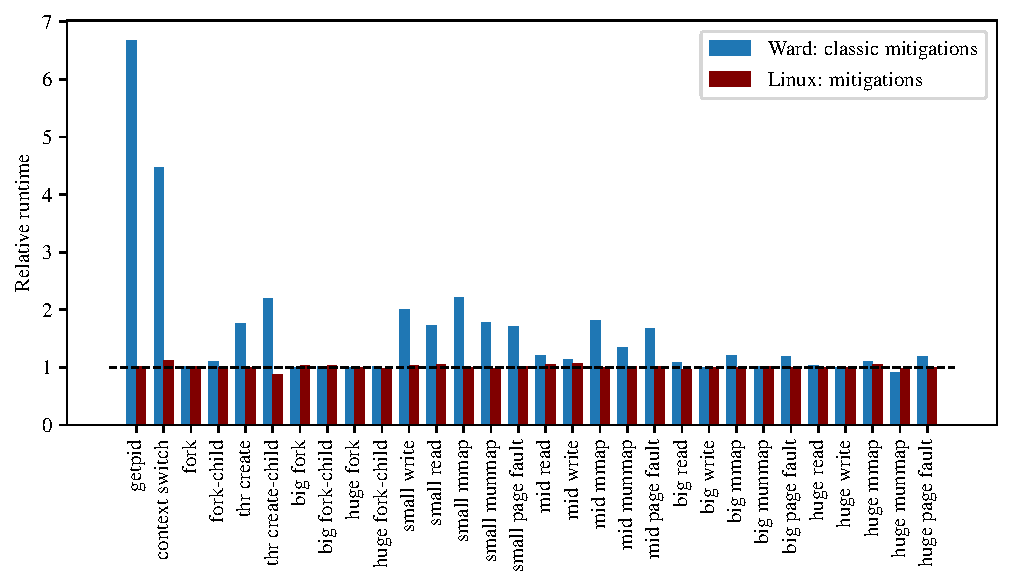
\includegraphics{results/ward_linux_overhead_lebench}
%%   \end{center}
%% \caption{Overheads for full mitigations for \sys and Linux}
%% \label{fig:ward_linux_slowdown}
%% \end{figure*}

%% The baselines for \autoref{fig:ward_linux_slowdown} are \sys and Linux
%% without mitigations. \autoref{fig:ward_linux} shows the relative
%% performance of \sys vs. Linux.

%% \fk{explain radixtree code to address big/huge mmap and fork.  issue:
%%   radix tree can merge 128 pages, but not merged more work (e.g., ref
%%   count) same per 512x128.  benchmarks does 10,000, merge per 128
%%   pages. increase fanout would allow us to do better.}



%% \begin{figure*}[t]
%%   \begin{center}
%%     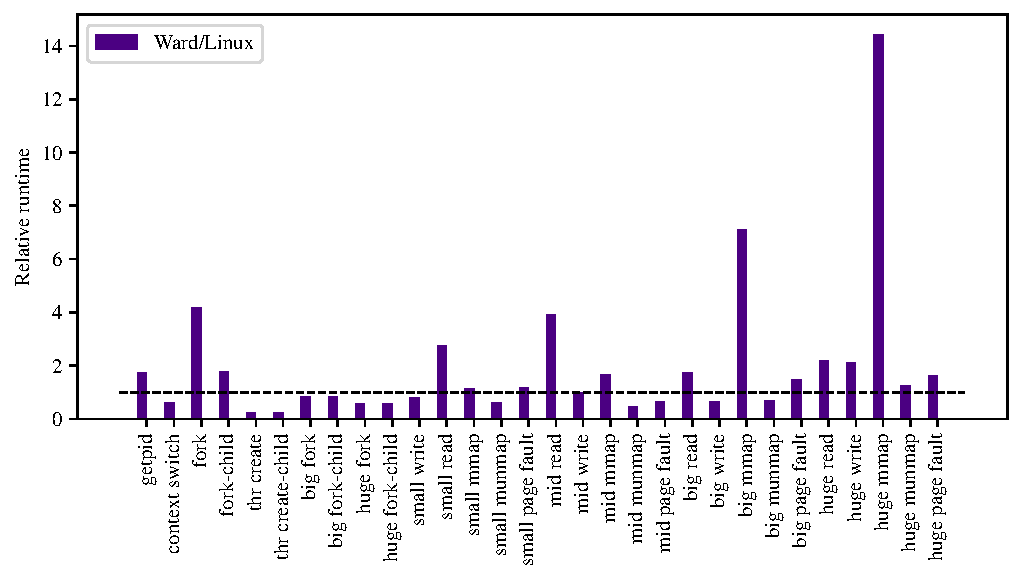
\includegraphics{results/ward_linux_lebench_no_mitigations}
%%   \end{center}
%% \caption{\sys relatative to Linux with no migitations.}
%% \label{fig:ward_linux}
%% \end{figure*}



%\section{Discussion}
\label{s:discussion}

\paragraph{Future vulnerabilities.}

It is likely that there are further transient
execution attacks either under embargo or yet to be discovered. Based on trends
in the existing attacks, we believe that \sys should be well positioned to
address them: so far, mitigations developed for Linux have been suitable to
directly copy into \sys. Since many need to run only at K domain entry/exit
instead of every user-kernel boundary crossing, the same defenses in \sys
might be cheaper to apply than they would be for Linux.

\paragraph{Linux.}

%% The results in \autoref{s:eval} shows that Ward's design can avoid
%% incurring the mitigation overhead for important system calls by executing
%% them in the Q domain without mitigation.  Although the evaluation involves
%% a research kernel with less features than a production kernel like
%% Linux,

We are optimistic that Ward's techniques could also benefit monolithic
production kernels for two reasons.
First, \sys and Linux are in the same ballpark in terms of system call
performance on \bench.  Out of the 30 microbenchmarks, \sys is faster than
Linux on 18 of them, and slower on 12.
%% Although the kernel designs are different in some
%% respects (and \sys is quite a bit simpler than Linux), this suggests
%% that the relative costs of mitigations on \sys are a reasonable proxy
%% for that on Linux.
Second, as shown in \autoref{fig:linuxslowdown} (\autoref{s:motivation})
Linux incurs a significant overhead for mitigations on \bench and that
overhead is in line with the overhead that \sys's Linux-style mitigations
incur on \bench (see
\autoref{fig:slowdown}).  Some systems calls experience more overhead in
\sys, because they implement less functionality (e.g., \texttt{getpid}),
but the corresponding calls in Linux also incur significant overhead.
Some systems calls in \sys have less overhead than Linux, because they are
not as efficient; for example, big and huge \texttt{mmap} in \sys requires
an update of its radix-tree VM data structures~\cite{clements:radixvm},
while Linux just inserts the new region into a list. Linux may see a
bigger pay for those system calls with \sys's design than \sys.

A question is how much effort is required to incorporate
\sys's techniques into a production kernel such as Linux.
%% To shed some
%% light on this question, we have started to modify the Linux kernel
%% to incorporate \sys's ideas.
Our preliminary efforts have proven
encouraging: we found that we could leverage existing infrastructure
for KPTI to maintain Q domain and K domain page tables.  We implemented
a \texttt{switch\_world} function in Linux, which switches to the K
domain and copies the Q stack to the K stack.  We modified the Linux
page-fault handler to call this function when it encounters a page
fault while running with the Q page table. This allows the Linux kernel
to run as normally with a transparent world switch on each system call.
We refactored the \texttt{struct task\_struct} into a Q-private and secret
part, allowing the \texttt{gettid} system call to run completely in the
Q domain.  This gives us some indication that the basic approach of \sys
could be made to work in Linux, although an open question is how to best
re-design the data structures in the Linux kernel to fit \sys's design.


\chapter{Related Work}
\label{s:related}

This thesis is motivated by the papers that show how secret kernel data
can be leaked through micro-architectural state, which started with the discovery of Meltdown~\cite{lipp:meltdown} and the original Spectre~\cite{kocher:spectre} variants.
These were rapidly followed by the discovery of more attacks targeting transient execution, including MDS~\cite{canella:fallout,schwarz:zombieload,schaik:ridl}, Speculative Store Bypass~\cite{horn:speculative-store-bypass}, and many others~\cite{bhattacharyya:smotherspectre,bulck:foreshadow,chen:sgxspectre,koruyeh:spectrersb,ragab:crosstalk,stecklina:lazyfp,schaik:cacheout,weisse:foreshadow-ng, bulck:lvi}.
Several survey papers were helpful by categorizing the known attacks~\cite{hill:survey,sok:transient,xiong:survey}.

We rely heavily on the mitigation work in the Linux
community~\cite{linux:vuln}. \sys adopts Linux's techniques and their
optimized implementation in the K domain.  \sys uses, for example,
Linux's \texttt{nospec} macro for bounds clipping,
\texttt{FILL\_RETURN\_BUFFER} to fill the return buffer, and retpoline.
\sys's hotpatching of its kernel text to remove retpolines in the Q
domain was inspired by Linux's \textsc{alternative}
macro~\cite{lwn:alternative}.

In addition to the software/microcode approach currently used by Linux and other other operating systems on older hardware, some of these attacks have been fixed in production hardware~\cite{intel:affected-processors}.
Meanwhile known hardware techniques for addressing others require more substantial changes~\cite{barber:specshield, weisse:nda, ainsworth:muontrap,yu:stt,yu:sdo}, generally by somehow delaying the use of speculative data until it is safe.
While such defenses are
more comprehensive, they have higher overheads that impact performance whenever
speculation occurs. By contrast, the \contract constrains speculation in a more
targeted way based on memory mappings. ConTExT also proposes constraining
speculation based on memory mappings, but introduces a new PTE bit to explicitly
mark pages that contain secret data~\cite{ConTExT}. \sys instead keeps secrets in
separate address spaces, and allows speculation after employing its defenses to
switch to the K domain.  Finally, SpecCFI proposes to enforce control-flow
integrity during speculative execution~\cite{koruyeh:speccfi}. This idea strengthens
Spectre defenses, and is complementary to \sys.

User-space sandboxing requires its own set of techniques.
Swivel~\cite{narayan:swivel} is a compiler framework which hardens WASM bytecode against attack, while
Firefox's and Chrome's WASM engines rely on Site Isolation~\cite{reis:site-isolation}.
Production JavaScript engines deploy more targeted mitigations like Pointer Poisoning and Index Masking~\cite{webkit:spectre-meltdown}, and also reduce the overall timer precision~\cite{mozilla:timer-precision, webkit:spectre-meltdown}.
Compiler techniques like Speculative Load Hardening~\cite{carruth:slh} ensure binaries are completely immune to Spectre, albeit at considerable overhead.

The Q page table is inspired by the shadow page table in
KAISER~\cite{gruss:kaiser} and KPTI~\cite{linux:kpti}. In Linux, when
a process executes in user space, the process runs with a shadow
page table, which maps only minimal parts of kernel memory: the kernel
memory to enter/exit the kernel on a system call. As soon as the process
enters the kernel, it switches to the kernel page table that maps all
of physical memory.  \sys, however, executes complete system
calls while running under the Q page table; this requires a significant
redesign of the OS kernel, which is a major focus of this work.

The use of virtual-memory to partition the kernel address space has a
long history in operating systems research.  One example is
Nooks~\cite{swift:nooks-tocs}, which runs device drivers in separate
protection domains with their own page table in kernel space to
provide fault isolation between drivers and the kernel.  Another
example is the use of Mondrian Memory Protection~\cite{witchel:mmp} to
isolate Linux kernel modules in different protection domains within
the kernel address space~\cite{witchel:mondrix}.  The most
recent example is Mike Rapoport's work on kernel address space
isolation~\cite{lwn:beyond-kpti} in Linux.  These designs use similar
techniques to introduce isolation domains within the kernel, but focus
on traditional attacks (e.g., code execution through a buffer overflow)
as opposed to transient execution.

%Flush Conflict~\cite{weber:osiris} automated discovery

Phoronix has conducted some of the most notable performance studies~\cite{phoronix:perf-zombieload, phoronix:two-years, phoronix:three-years}. A few other groups have conducted studies~\cite{nikolay:meltdown-spectre-performance,prout:measuring-spectre-meltdown} but those predate the most recent attacks.
The Linux community has paid close attention to the cost of mitigations throughout, including for IBRS~\cite{linus:ibrs-rant},  KPTI~\cite{gregg:kpti-perfromance}, and MDS~\cite{phoronix:perf-zombieload}.
Their work has played a role in both understanding and driving down the performance overheads.

% Several survey papers~\cite{hill:survey,sok:transient,xiong:survey} classify attacks but not their performance impact, while LEBench~\cite{ren:lebench} explored how mitigations impacted performance across kernel versions.

% Where this work stands out is by looking at many different generations of CPUs and characterizing the performance impacts of the set of mitigations deployed in practice.

% Uses size information to avoid spectre
% https://www.cs.columbia.edu/~mtarek/files/preprint_ISCA21_NoFAT.pdf

% MuonTrap. A hardware approach to preventing spectre attacks by preventing speculative accesses from ever entering the cache. 5% slowdown on SPEC, but actually a speedup on PARSEC due to their tiny but fast L0 cache.
% https://arxiv.org/pdf/1911.08384.pdf

% Speculative Data-Oblivious Execution. Hardware approach to preventing spectre attack. Builds on Speculative Taint Tracking.
% [SDO] https://iacoma.cs.uiuc.edu/iacoma-papers/isca20_2.pdf
% [STT] https://www.cs.tau.ac.il/~mad/publications/micro2019-stt.pdf
%
% Contains a good summary of related work on hardware defenses for speculative execution.

% Mitigation list on Intel Processors.
% https://software.intel.com/content/www/us/en/develop/topics/software-security-guidance/processors-affected-consolidated-product-cpu-model.html

% Swivel: Hardening WebAssembly against Spectre
% https://www.usenix.org/system/files/sec21-narayan.pdf

% DOLMA: Hardware approach with 10-40% but more complete coverage of attacks, including those targeting registers
% https://www.usenix.org/conference/usenixsecurity21/presentation/loughlin

% Rage Against the Machine Clear. Study of machine clears as a root cause for attacks. Also has a good list of attacks in related work section (plus list 3 survey papers on it)
% https://www.usenix.org/system/files/sec21-ragab.pdf


%% A kernel-organizational view of \sys is that the K domain is a
%% microkernel that provides services to Q domains~\cite{liedtke:sosp95},
%% but all running in kernel mode. Alternatively, one can view the K
%% domain as a hypervisor multiplexing several virtual machines that each
%% run an application with its Q domain~\cite{bugnion:disco,barham:xen}.
%% In both views, the interface between the Q and the K domains is more
%% porous than a microkernel or hypervisor interface: parts of data
%% structures of the K domain are directly mapped into Q domains to avoid
%% world switches.

%% other related work:

%% %https://www.microsoft.com/en-us/research/wp-content/uploads/2017/08/cloak_sec17.pdf

%% %https://www.usenix.org/system/files/conference/usenixsecurity18/sec18-dong.pdf

%% T-SGX (Shih, NDSS 2017)

%% architectural changes (e.g., removing side channel, avoiding resource
%% sharing)

%% Yan, InvisiSpec

%% oo7: low-overhead defense against spectre attacks via binary analysis



\chapter{Discussion and Future Work}
\label{s:discussion}
The ongoing impact to performance of transient execution attacks is continuing to decline on newer processors, and on some workloads isn't even measurable at all.
Watching the stream of new transient execution attacks being published might not give this impression, but that comes from looking at the quantity of attacks independent of their performance drain.

One aspect in particular that is easily overlooked is that production operating systems don't try to provide perfect isolation in the first place.
This is a challenge for the security community because it is much harder to model, but a tremendous opportunity to the systems community that can ignore low severity side channels (or accept incomplete fixes for more severe ones).
It means that a proposed method by a security researcher to mitigate a specific side channel attack might be deemed excessive by the developer community.

One example is disabling hyperthreading.
While theoretically necessary to mitigate certain attacks, Linux by default choses to just ignore that advice and run mutually untrusting processes on adjacent hyperthreads.
An even more pronounced case is Spectre V1: the only way to be 100\% sure that no gadgets are present is to insert speculation barriers of some sort after every single branch in the kernel, because there isn't a programmatic way to know which are vulnerable.
Instead Linux developers just annotate all the specific code sequences they can find to prevent them from being exploited.
From a theoretical sense this is deeply unsatisfying since there are almost surely places that have been missed.
However, the constant stream of memory safety and logic bugs being discovered in the kernel makes any comparatively difficult to exploit Spectre vulnerabilities of limited concern.

If strong security against transient execution attacks is needed, critical applications can achieve much higher guarantees of isolation by running on dedicated hardware because transient execution attacks only work if the attacker and victim are sharing the same physical machine.
This makes them immune even to attack variants that haven't been discovered yet, but naturally comes with its own downsides.
The combination of added cost, reduced utilization, or degraded usability mean that this approach is usually reserved only for applications that absolutely require it.

It is also worth considering performance impacts in context.
The Zen 3 processor we experimented with might look like it has the worst overhead from Speculative Store Bypass Disable, but that is only on relative terms.
In fact, it is so much faster than any of the other machines we tested on the benchmarks, to the point that with SSBD enabled it outperformed all the other processors when they had SSBD disabled.
That partly comes down to clock speed, but also the generational improvement in CPUs, which almost invariably exceeds the at this point roughly 3\% overhead that OS-level mitigations cause to syscall workloads.

With the context discussed so far, the major area most applicable for future work is JavaScript isolation.
Across all the processors we studied, overheads from mitigations have been high and unchanging across processor generations.
A big chunk of JavaScript overhead is from SSBD, which may be solvable by hardware at low cost or avoided by simply not enabling the mitigation.
However, that requires drawing attention to it: most public documentation emphasizes that SSBD isn't used by default and neglects to mention that critical applications like web browsers frequently run with it enabled.

The second facet of possible future work is addressing Spectre V1 from sandboxed JavaScript code.
JIT compilers can readily insert appropriate bounds check instructions and speculation barriers to prevent the common variants of the attack.
However, existing processors are not tuned to accelerate these code patterns, so the cumulative impact of running them thousands or millions of times can have a detrimental impact on performance.
This doesn't need to be the case.
The computer architecture community has already studied ways for a CPU to perform memory operations without introducing Spectre gadgets~\cite{ainsworth:muontrap,yu:stt,yu:sdo}.
Those techniques can be painfully slow when applied to every memory operation in a program, but could be far more reasonable when applied only to memory instructions flagged by the JIT.


\chapter{Conclusion}
%\section{Conclusion}
\label{s:concl}

This thesis assesses the evolution of performance penalties for
mitigations against transient execution side-channel attacks by
measuring their overheads across several generation of Intel and AMD
CPUs, and introduces the \sys kernel design which eliminates as much
as half this overhead on OS heavy workloads.

Although the time passed since the first mitigations is short,
we observe a few trends: 1) on an OS-intensive workload the
overhead of mitigations has declined from over 30\% on our oldest
processor to under 3\% on the most recent CPUs; and 2) JavaScript
sandboxing stresses different mitigations, whose overheads are
significant and unchanged across successive generations.

A further analysis of individual mitigations shows that the hardware
improvements in successive generations have reduced the overhead of
some mitigations to something small, while the overheads for Spectre
V1 and V2 mitigations haven't changed across processor generations and
are significant.  We speculate, however, that it should be possible to
reduce these overheads of these mitigations with hardware changes too;
for example, the Spectre V1 mitigation has a recognizable pattern of a
conditional move followed by a load instruction, which could be
detected by hardware to trigger special handling.

%The \contract
%allows hardware to speculate on many values (but not the values of
%page table entries) and provides software with a mechanism to prevent
%leaking secrets through micro-architectural state.  
The \sys design
shows how \contract can be used to reduce the performance costs of
mitigations on system calls using per-process Q domains and global K
domains.  \sys transparently switches from Q- to K-domain through page
faults, uses temporary mappings to access unmapped physical pages, and
splits data structures into public and private parts.  An evaluation
shows that \sys can run the microbenchmarks of \bench with small
performance overhead compared to a kernel without mitigations: for
18 out of 30 \bench microbenchmarks, \sys's performance is within 5\%
of the performance without mitigations.
On Broadwell, \sys overall has a geometric mean slowdown of 16\% on \bench compared to 32\% for Linux.
% Although \sys is research kernel, we are hopeful that its
% ideas can carry over to production monolithic kernels.
Although \sys is research kernel, we are hopeful that the ideas of this thesis can drive further progress in production kernels and web browsers.


\pagebreak
\bibliography{n-str,paper,n,n-conf}{}
\bibliographystyle{plain}

\end{document}
